
\chapter{Experiments, Results and Analysis}\label{ch:experiment}
This chapter presents the experiments conducted to fine-tuning an umbrella Arabic DID, then assessing 
its robustness and adaptability. The results are analysed and the system setup for each of the experiments are detailed in Chapter \ref{ch:methodologies}. 
The full, detailed results are provided in Appendix \ref{sec:appA}. 

\section{Preliminary experimentation}
Prior to streamlining the final system pipeline for the Umbrella DID some preliminary testing was performed. These 
experiments provided vital information that informed some desgin choices for the final system pipeline. As well as confirming 
some assumptions made when undertaking this thesis. 
\subsubsection*{Testing SpeechBrain LID performance on Arabic Dialects}
An out of the box Python package that perform's langauge identification (LID) is the SpeechBrain package. 
The system has a ECAPA-TDNN architecture which is composed primarily of convolutional and residual layers. The 
LID was trained using CommonLanguage, a curated subset of data from the open source dataset CommonVoice. The dataset is sourced 
from voluntarily submitted audio files. In order to get an understanding of the gaps in LIDs in identificating dialectal Arabic as Arabic, 
the ADI17 dataset was run through SpeechBrain's LID. The LID had an overall accuracy of 87.69\%.
Investigating the LID's performance on the umbrella dialects it identified Egyptian (EGY) with the highest accuracy of 90.72\%, 
Gulf (GLF) with the lowest accuracy of 85.77\% and the dialects were most likely to be misidentified as Somali (so) or Hebrew (iw). 
Breaking down that performance into the regional dialects Jordian (JOR) Arabic was identified as Arabic with the highest level of accuracy at 95.98\% and  
Yemen (YEM) Arabic was identified with the lowest accuracy of 81.58\%. Thereby, showing that despite LID systems working well at identifying dialectal Arabic as Arabic there is still room for improvement. Having a specialised Arabic DID could improve 
both LID systems and other speech systems. 

\subsubsection*{Amount of Training files}
In order to determine what a reasonable amount of data files were for performing basic training of the 
the DID system a preliminary test was conducted. The resources allocated for the experiment were 2 GPUs, 16 CPUs and 92GB of memory. 
Wav2vec 2.0 base was used as the pretrained model and the audio was truncated to 5 seconds. Training with 
50, 100, 500 and 1000 files per dialect was tested, their validation accuracies were 27.29\%, 32.06\%, 34.30\% and 33.51\% respectively. Additionally, 
the runtime on average was 1hr and did not fluctuate greatly when the files were increased. From this experiment it was determined that training with 500-1000 files per dialectal group 
would be sufficient. 700 files per dialect was chosen in further testing to be the default training amount. 
\subsubsection*{Batch Size}
Another variable that was experimented with to determine a reasonable base amount was batch size. Batching is when training samples are grouped together to be processed parallel to one another 
at an iteration. Out of the pretrained models that will be experimented with in later tests, the model with the largest amount of parameters to train and thereby requires the most amount of working memory is 
XLSR. So the experiment was conducted with XLSR Arabic with 2 GPUs, 16 CPUs, 92GB of memory and the audio was truncated to 10 seconds. 
Using 500 training files the batch sizes 8, 20, 40 were tested. The maximum validation accuracy was 44.4\%, 44.6\% and 43\% respectively. While their runtimes were 2.04hrs, 1.08hrs and 1.04hrs.
So, it was determined that the batch size didn't significantly effect the performance of the system, although larger batch sizes did help reduce runtime. It was also confirmed that the larger batch sizes required significantly larger amounts of memory to process, 
with the largest batch size that could be used without the system running out of working memory being 40. A batch size of 40 was then to be used as the default training amount in further experimentation. 
\section{Fine-Tuning an Umbrella Arabic DID}\label{sect:finetuneUmbDID}
The focus of the experiments in this section is to determine the design choices and factors 
which will produce the highest performance Umbrella Dialect Arabic DID. The four umbrella dialects are North Afriacan (NOR), Egyptian (EGY), 
Gulf (GLF) and Levantine (LEV). The breakdown of these groupings and the data used can be read in Section \ref{sect:dataset}. 
\subsection{Assessment of Performance of Pretrained Models}\label{sect:pretrainExp}
The first formal experiment conducted on the umbrella Arabic DID was trialing the use of different pretrained models. The resources allocated for these tests were 3 GPUs, 
24 CPUs with 138GB of memory allocated. The results are presented in the table \ref{tab:f1pretrain}, figure \ref{fig:pretrainsum} and figure \ref{fig:xlsrcolourmap}. 
The aims of experimenting with different pretrained models was to determine:
\begin{itemize}
    \item{The effect of structure. }
    \item{The significance of using a diverse range of languages in the training data.
    }
    \item{The adaptability of models fine-tuned for similar downstream tasks. 
    }
\end{itemize}
The two base structures tested in this experiment were Hubert and Wav2Vec 2.0, with more details about their architecture provided in the Section \ref{sect:trans}. 
Hubert outperformed the base wav2vec in all significant metrics and had a weighted average F1-Score that was 15\% greater than it. Although, compared to Wav2Vec 2.0, 
Hubert does not have many variants and so, further testing was conducted on wav2vec variant models. 
The next objective of this experiment was to compare the base wav2vec with 
XLSR, a variant trained with 53 languages and a version of XLSR which had been further fined tuned with Levantine Arabic data. The highest performance was from XLSR Arabic with 
a weighted average F1-Score of 63\%, 14\% higher than the base wav2vec and 45\% higher than the base XLSR. An interesting behavior of the base XLSR was it's inability to 
identify Egyptian or Levantine Arabic, predicting the data was Gulf (GLF) Arabic  91.96\% of the time. This bias towards Gulf Arabic can be seen in Figure \ref{fig:xlsrcolourmap} and 
is most probably due to biases within the pretraining dataset. With the data used pretrain XLSR being from the Gulf region or Modern Standard Arabic (MSA) which is most similar to Arabic from the Gulf region.
Finally, models which had been fine-tuned for similar downstream tasks were tested. Comparing wav2vec fine-tuned for LID and SID tasks against the base model, both of the downstream task models outperformed the base wav2vec. 
The wav2vec SID had the highest F1-Scores with a weighted average F1-Score 16\% greater than the base wav2vec and comparable to XLSR Arabic. Looking at the results for North African (NOR) Arabic 
wav2vec SID marginally outperformed XLSR Arabic by 2\%. The wav2vec LID also had comparable results to Hubert performing marginally better at identifying North African (NOR) and Gulf (GLF) dialects. 

This experiment also gave an indication of the dialects the system excels or struggles at identifying. It was found that across all the pretrained model types 
the system was able to identify North African with the greatest proficiency and Levantine with the least.  

Ergo, from this experiment it was found that using a pretrained model that was already fine-tuned with a similar dataset or for a similar downstream task was more 
effective than using a base pretrained model. For further experimentation the XLSR Arabic pretrained model was chosen to be used based on these results, as the features used to differentiate the  
dialects were less likely to be the acoustic features or features of the speaker compared to the wav2vec SID model. 

\begin{table}[h!]
    \centering
    \caption{Umbrella DID F1-Score Breakdown of each Dialect for Pretrained Models}
    \label{tab:f1pretrain}
    \begin{tabular}{|l|l|l|l|l|l|l|l|} 
    \hline
    \multicolumn{8}{|c|}{\textbf{F1-Score (\%)}}                                                                                                                                                 \\ 
    \hline
                                                       & Hubert & XLSR & XLSR Arabic & wav2vec & wav2vec sid & wav2vec lid & \textbf{Average}  \\ 
    \hline
    NOR                                                & 67     & 30        & 70          & 50               & 72          & 68          & 60 \\ 
    \hline
    EGY                                                & 64     & 0         & 64          & 48               & 65          & 60          & 50 \\ 
    \hline
    GLF                                                & 61     & 42        & 62          & 54               & 60          & 63          & 57 \\ 
    \hline
    LEV                                                & 56     & 0         & 54          & 35               & 53          & 51          & 42 \\ 
    \hline
    \textbf{Weighted Average} & 62     & 18        & 63          & 47               & 63          & 61          &                                                       \\
    \hline
    \end{tabular}
    \end{table}


    \begin{figure}[h!]
        \centering
        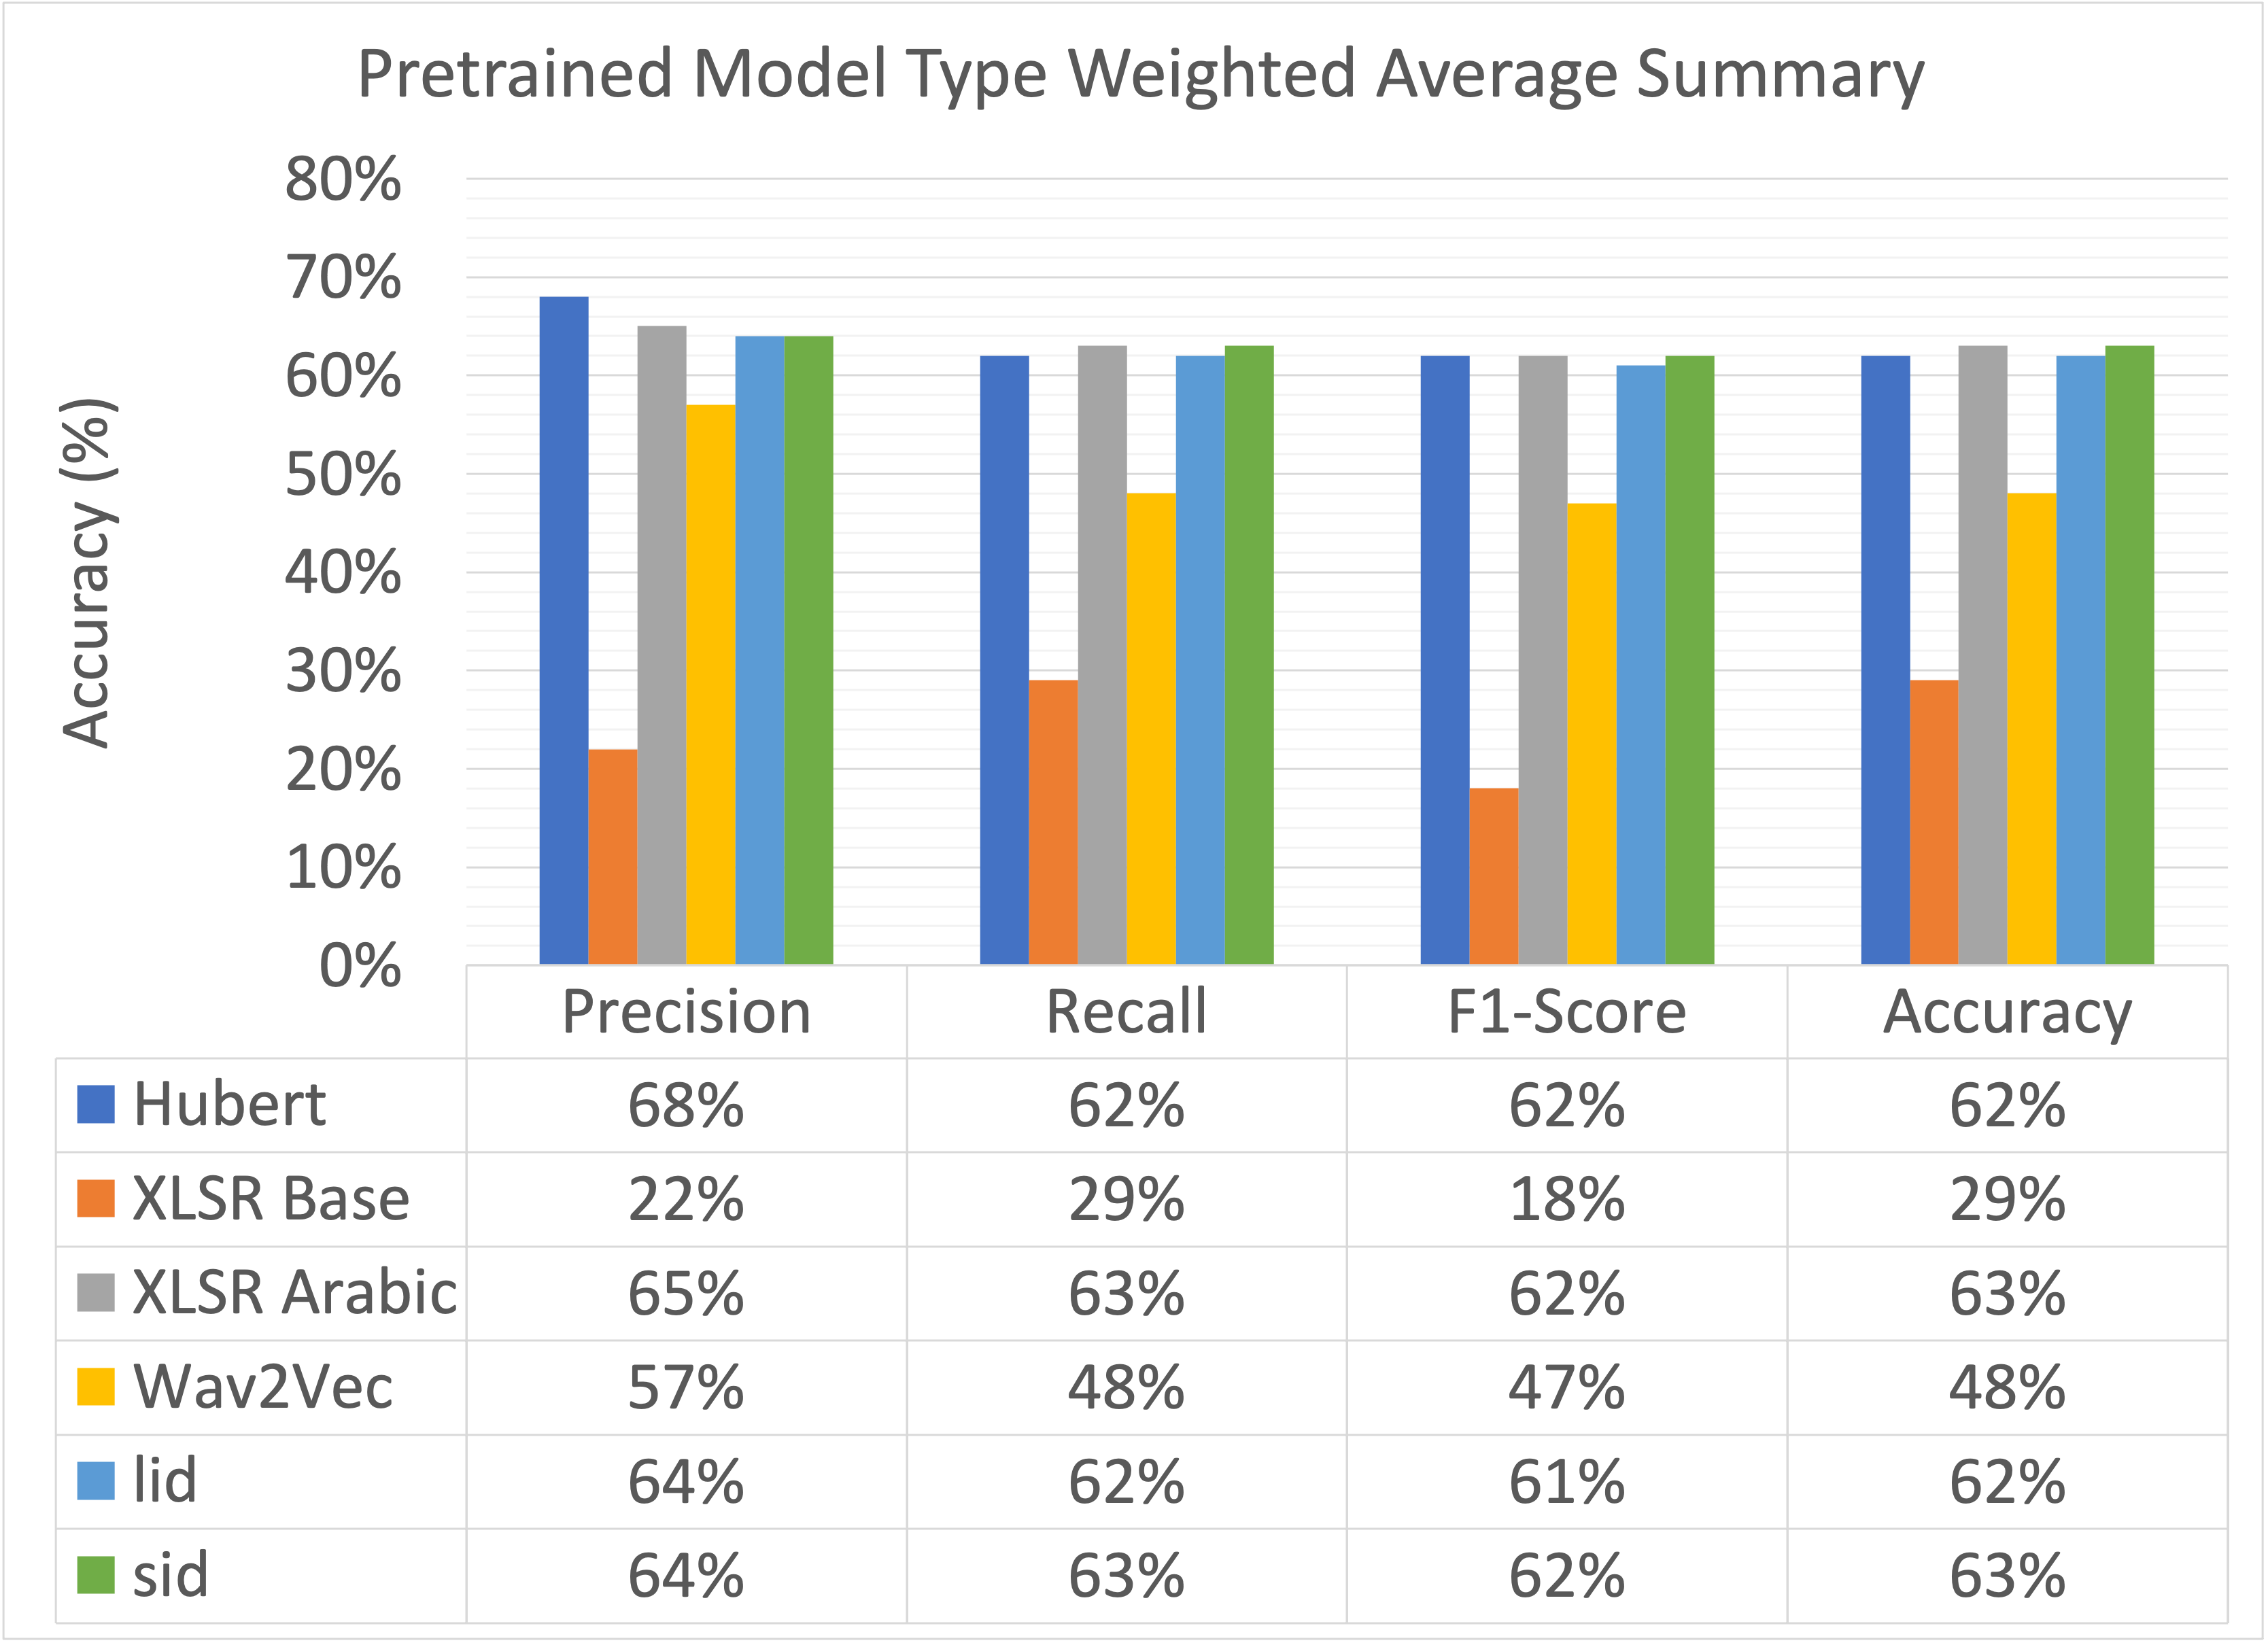
\includegraphics[width=\textwidth]{plots/pretrainedModelSum.png}
        \caption{Plot comparing key metrics for different pretrained models.}
        \label{fig:pretrainsum}
    \end{figure}

    \begin{figure}[h!]
        \centering
        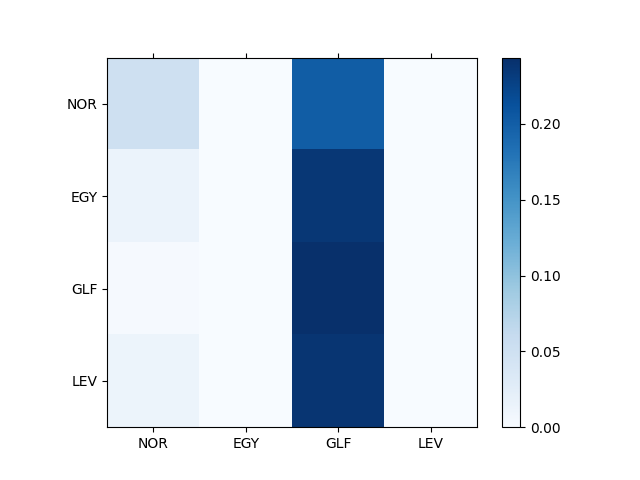
\includegraphics[width=\textwidth]{appendix/ADI17-xlsr-basic-norm.png}
        \caption{XLSR Normalised confusion Matrix Colour map.}
        \label{fig:xlsrcolourmap}
    \end{figure}

\pagebreak 
\subsection{Exploring Noise filtering}\label{sect:noiseExp}
The ADI17 dataset, is sourced from Youtube clips, many of the audio clips contain background noise. As discussed in 
Section \ref{sect:dataset} adding noise filtering can increase the performance of a DID. The focus of this experiment was 
to test two filtering methods against the performance of an umbrella DID with no filtering performed on the dataset. The 
tests were performed with XLSR Arabic as the pretrained model, the audio files truncated to 10 seconds and 
The first method tested was using the Python package noise reduce. The package over filtered the audio clips, reducing the clarity 
of the speaker as seen in a sample utterance waveform in figure \ref{fig:Noise} and had a final accuracy of 53.3\%, 10\% less than the unfiltered 
dataset. 
The second method tested was a Butterworth bandpass filter with a lower cutoff frequency of 50Hz and an upper cutoff frequency of 500Hz. The 
frequencies were chosen with the aim to cut off any sound outside the human vocal range. The bandpass filter also didn't perform well in comparison to the 
unfiltered signal with an accuracy of 43.3\%, 20\% less than the filtered signal. This reduced accuracy is also due to the distortions filtering causes to the 
audio signals as shown in figure \ref{fig:Bandpass}. 
Thereby, it was found that despite the literature suggesting noise filtering would improve the umbrella DID's performance it was 
not found as an effective strategy. 

\begin{table}[h!]
    \centering
    \caption{Effect of Noise Filtering on Final Accuracy}
    \begin{tabular}{|l|c|} 
    \hline
    \textbf{Filtering Method} & \textbf{Accuracy(\%)}  \\ 
    \hline
    Noise Reduce Package      & 53.3                   \\ 
    \hline
    Band pass Filter           & 43.3                   \\ 
    \hline
    No Filter                 & 63.2                   \\
    \hline
    \end{tabular}
    \end{table}

\begin{figure}[H]
    \CommonHeightRow{
        \begin{floatrow}[2]
            \ffigbox[\FBwidth]
            {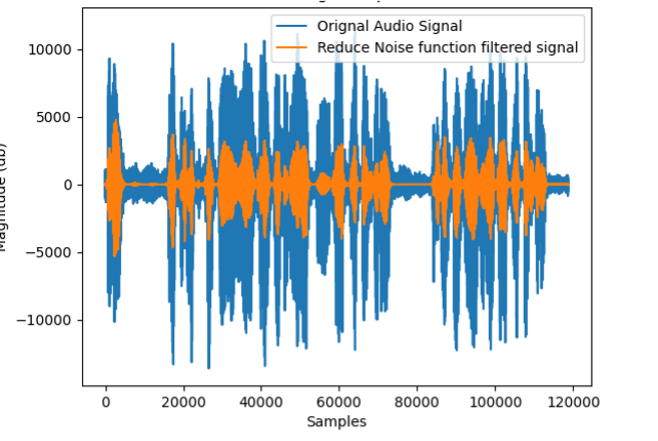
\includegraphics[height=6cm]{plots/reduceNoise.png}}
            {\caption{Sample Utterance Filtered \newline using Reduce Noise Package}}\label{fig:Noise}
            \ffigbox[\FBwidth]
            {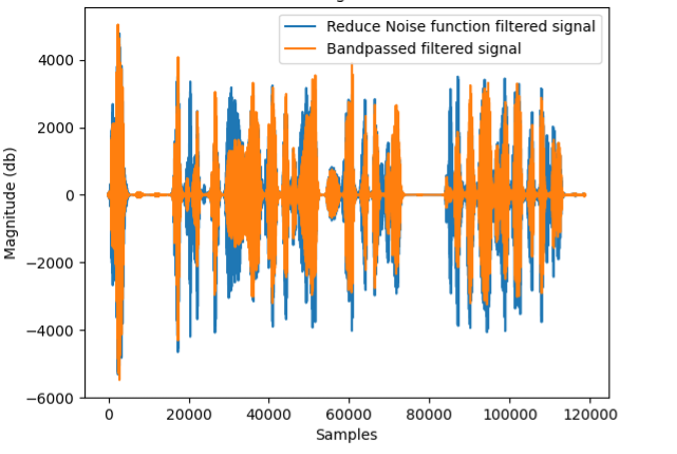
\includegraphics[height=6cm]{plots/Bandpass.png}}
            {\caption{Sample Utterance Filtered \newline  using Bandpass Filter}}\label{fig:Bandpass}
        \end{floatrow}}
\end{figure}


\subsection{Effect of Utterance Length}\label{sect:uttExp}
This experiment aimed to compare the performance of the umbrella DID with varying utterance lengths to find the 
minimum acceptable training utterance length. The training was performed with 3 GPUs, 24 CPUs with 138GB of memory 
and 500 files allocated per dialect. The utterances within the dataset range from 10 - 25s, a script was written to select files with audio lengths greater than or equal to 10s for the medium utterance length test 
and then greater than or equal to 20s for the long utterance length test. The files were then truncated to the specified training lengths of 5s, 
10s or 20s. Analysing the results in the Table \ref{tab:f1utter} the long and medium utterances had comparable performances. The longer utterances  
outperformed both short and medium utterances for most of the F1-Scores. With a weighted average F1-Score of 59\% it was 8\% greater than the medium utterances and 26\% greater than the short. 
Although, for the North African (NOR) dialect the medium utterances marginally performed better with an F1-Score of 57\% compared to the long utterance's 53\%. Looking at the 
confusion matrices colour maps shown in figures \ref{fig:medium} and \ref{fig:long}, the long utterances were more likely to be misidentified as Egyptian (EGY). 
Considering the runtimes of the medium and long utterance training segments shown in figure \ref{fig:uttsum}. Training with the long utterances have a significantly longer 
runtime demand of 7.36hrs compared to the medium's 1.13hrs. So, it was found that longer training utterances overall produced a higher performing DID but need significantly 
more resources to train. It was decided for further testing, particularly with more complex network structures and more fine-tuning layers that the performance of using medium clips 
had sufficient performance. 

\begin{table}[h!]
    \centering
    \caption{F1-Score for Varying Utterance Lengths.}\label{tab:f1utter}
    \begin{tabular}{|l|l|l|l|l|} 
    \hline
                     & \multicolumn{4}{c|}{\textbf{F-1 Score (\%)}}               \\ 
    \hline
                     & Short (5s) & Medium (10s) & Long (20s) & \textbf{Average}  \\ 
    \hline
    NOR              & 24         & 57           & 53         & 44.7              \\ 
    \hline
    EGY              & 48         & 56           & 58         & 54                \\ 
    \hline
    GLF              & 30         & 50           & 62         & 47.3              \\ 
    \hline
    LEV              & 30         & 41           & 63         & 44.7              \\ 
    \hline
    \textbf{Weighted Average} & 33         & 51           & 59         &                   \\
    \hline
    \end{tabular}
    \end{table}


    \begin{figure}[h!]
        \centering
        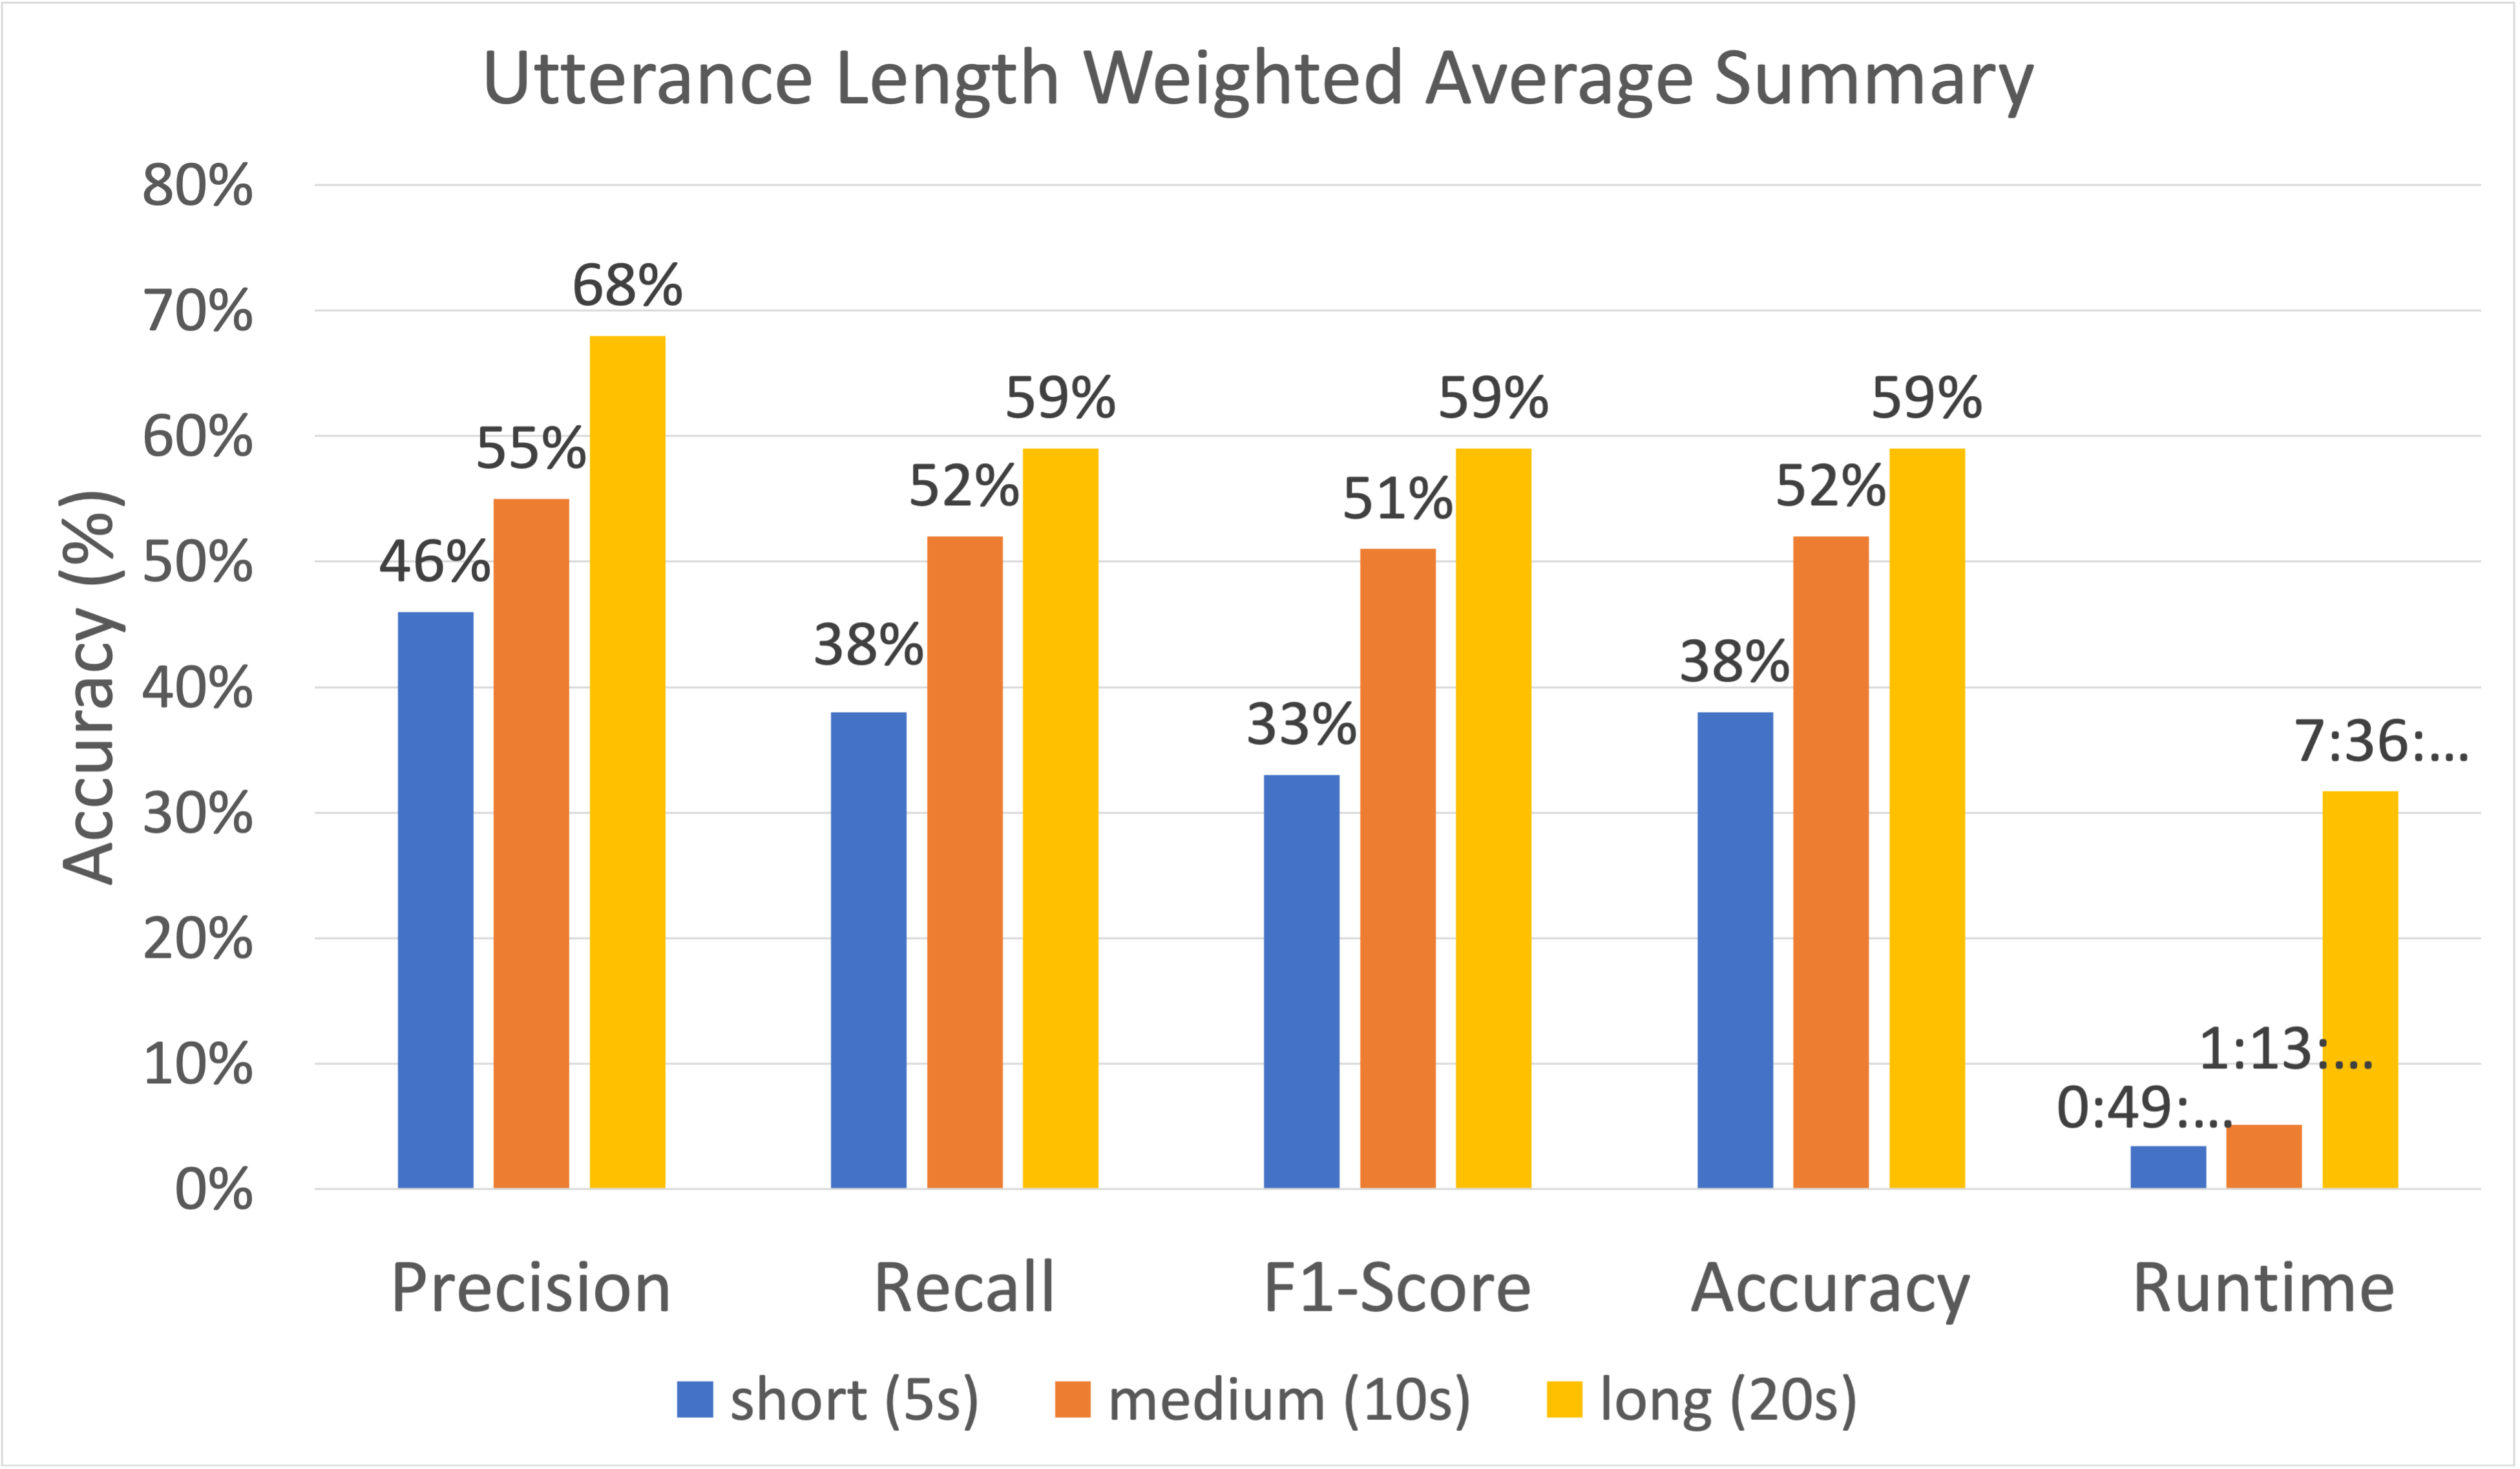
\includegraphics[width=\textwidth]{plots/utteranceLengthSum.png}
        \caption{Plot comparing key metrics varying training utterance lengths.}
        \label{fig:uttsum}
    \end{figure}

    \begin{figure}[h!]
        \CommonHeightRow{
            \begin{floatrow}[2]
                \ffigbox[\FBwidth]
                {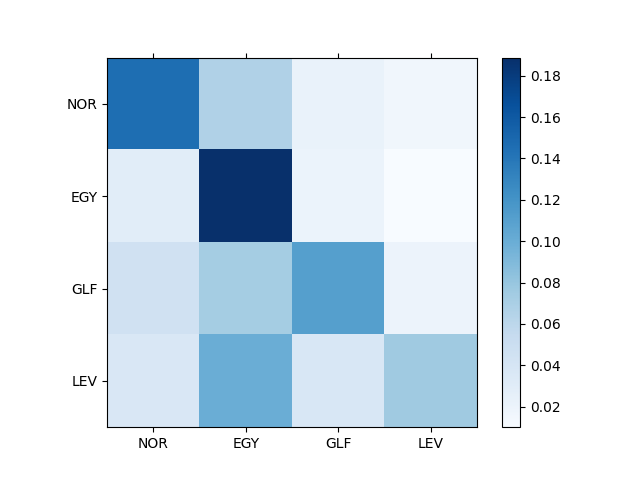
\includegraphics[height=6cm]{plots/ADI17-xlsr-medium-norm.png}}
                {\caption{Medium Utterances(10s)\newline Normalised Confusion Matrix Colour Map.}}\label{fig:medium}
                \ffigbox[\FBwidth]
                {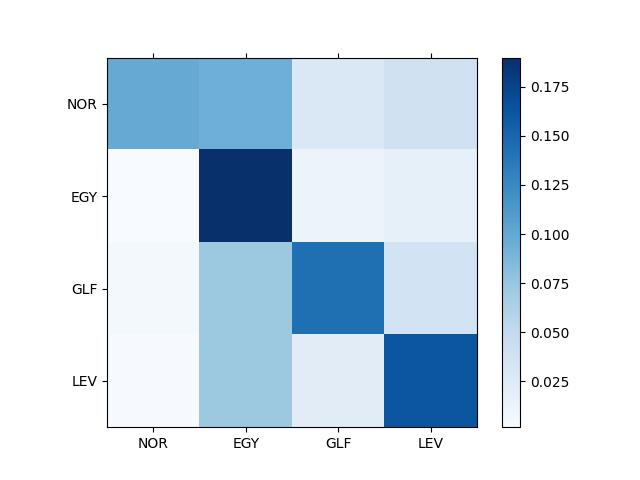
\includegraphics[height=6cm]{plots/ADI17-xlsr-long-norm.png}}
                {\caption{Long Utterances(20s)\newline Normalised Confusion Matrix Colour Map.}}\label{fig:long}
            \end{floatrow}}
    \end{figure}
\pagebreak 
\subsection{Fine-tuning with addition of a Downstream Model}\label{sect:downExp}
The aim of this experiment was to explore the possibility of enhancing the performance of the umbrella DID through 
the addition of a downstream model. The downstream models tested in this experiment structure is explained in Section \ref{sec:down}. The downstream models were inserted 
into a XLSR Arabic model and the weights from fine-tuning the model without the downstream model were loaded into the model when it was initalised. The training was performed with 3 GPUs, 24 CPUs with 138GB of memory 
and 700 files allocated per dialect.The LSTM performs poorly in all metrics as seen in the Figure \ref{fig:downSum}, classifying all the test files as Gulf with a F1-Score of 40\% as seen in the Table \ref{tab:f1scoredown}. 
The DNN structures outperform the LSTM but underperform compared to having no downstream model at all. Comparing the DNN models of varying layers and more complexities, the simplest 3 layer DNN performs the best overall with a weighted average F1-Score of 55\%. 
The 4 layer DNN has a marginally higher F1-Score than the 3 and 6 layer for North African (NOR) and Levantine (LEV) dialects. Whilst the results for the 
6 layer DNN are comparable to the 3 layer but with lower F1-Scores for Gulf (GLF) and Levantine (LEV) dialects. 

Analysing the Figure \ref{fig:downLoss}, it can be seen compared to having no downstream model, the model with a DNN structure has a steep 
decrease in it's training loss and increase in its validation loss. The trends in its loss over the epochs show that adding a DNN structure leads to overfitting 
during the fine-tuning process. So, it can be concluded from these findings that adding a downstream model adds unnecessary complexity to the system 
causing overfitting and decreasing the performance of the DID.  

\begin{table}[h!]
    \centering
    \caption{F1-Score of Varying Downstream Models}\label{tab:f1scoredown}
    \begin{tabular}{|l|l|l|l|l|l|} 
    \hline
                              & \multicolumn{5}{c|}{\textbf{F1-Score (\%)}}                              \\ 
    \hline
                              & DNN 3 layers & DNN 4 layers & DNN 6 layers & LSTM & No Downstream Model  \\ 
    \hline
    NOR                       & 64           & 66           & 64           & 0    & 70                   \\ 
    \hline
    EGY                       & 51           & 32           & 51           & 0    & 64                   \\ 
    \hline
    GLF                       & 57           & 56           & 53           & 40   & 62                   \\ 
    \hline
    LEV                       & 50           & 52           & 48           & 0    & 54                   \\ 
    \hline
    \textbf{Weighted Average} & 55           & 52           & 54           & 10   & 62                   \\
    \hline
    \end{tabular}
\end{table}

\begin{figure}[h!]
    \centering
    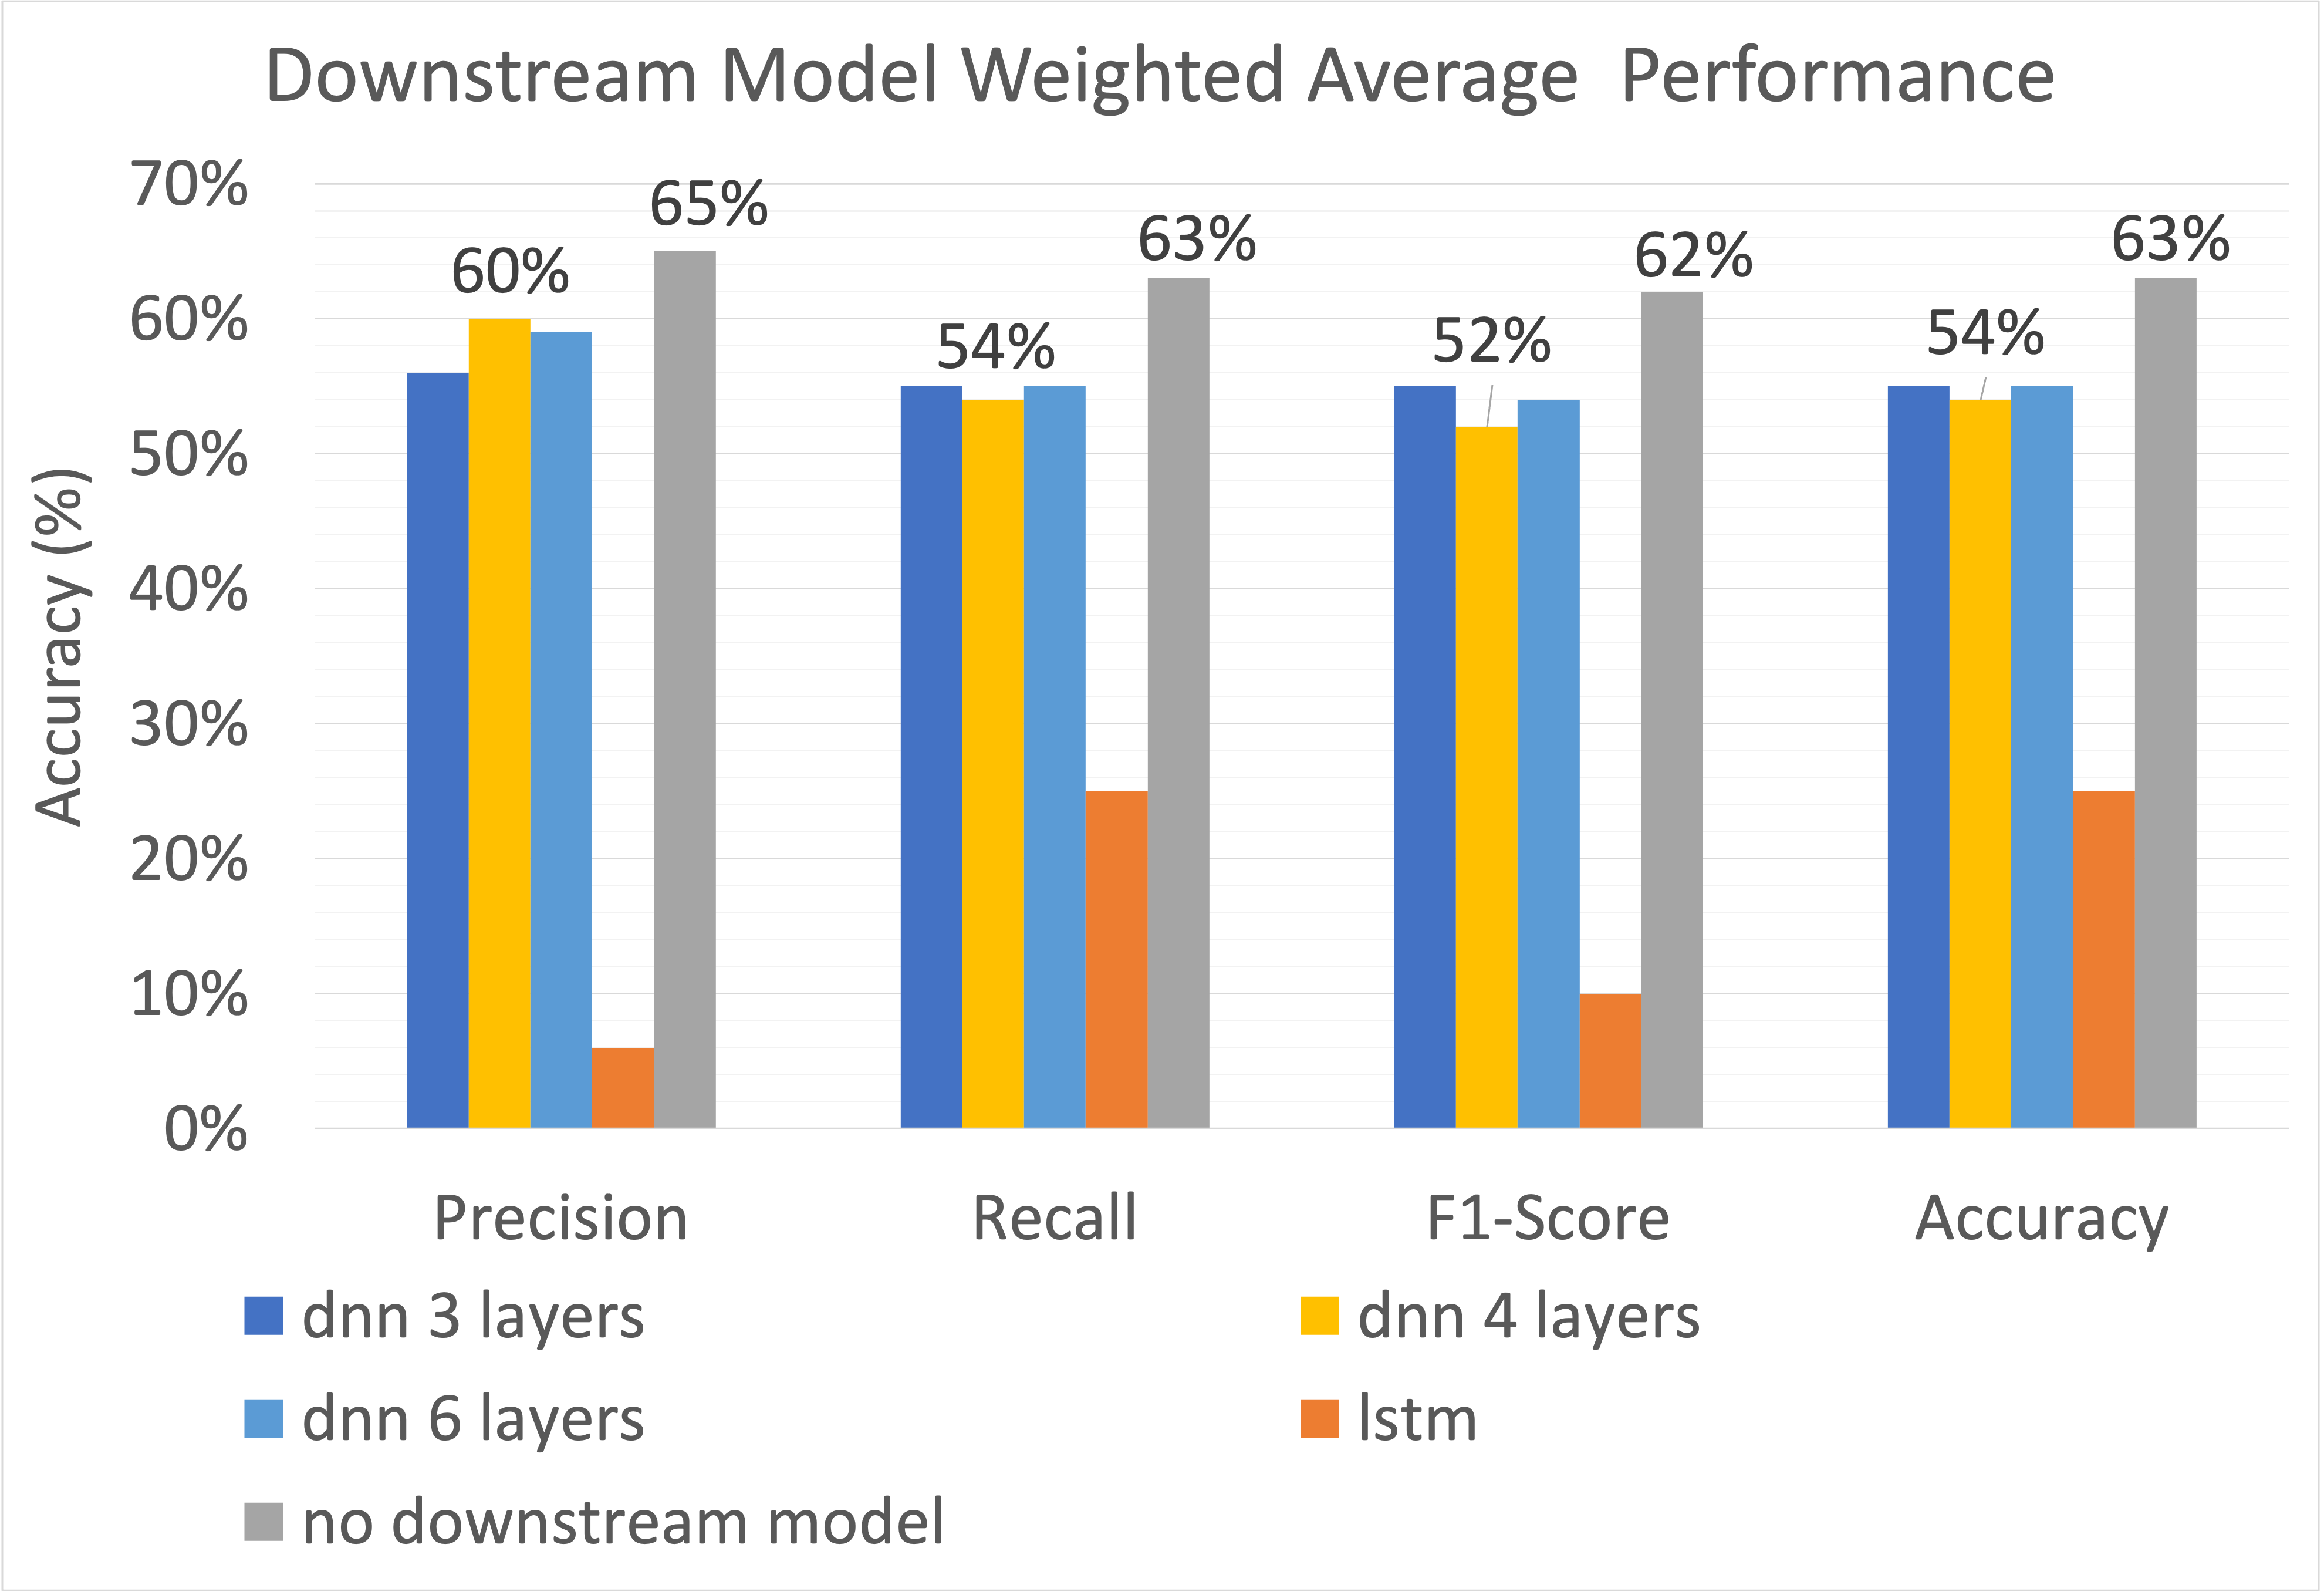
\includegraphics[width=\textwidth]{plots/downstreamSum.png}
    \caption{Downstream model Summary of key metrics.}
    \label{fig:downSum}
\end{figure}

\begin{figure}[h!]
    \centering
    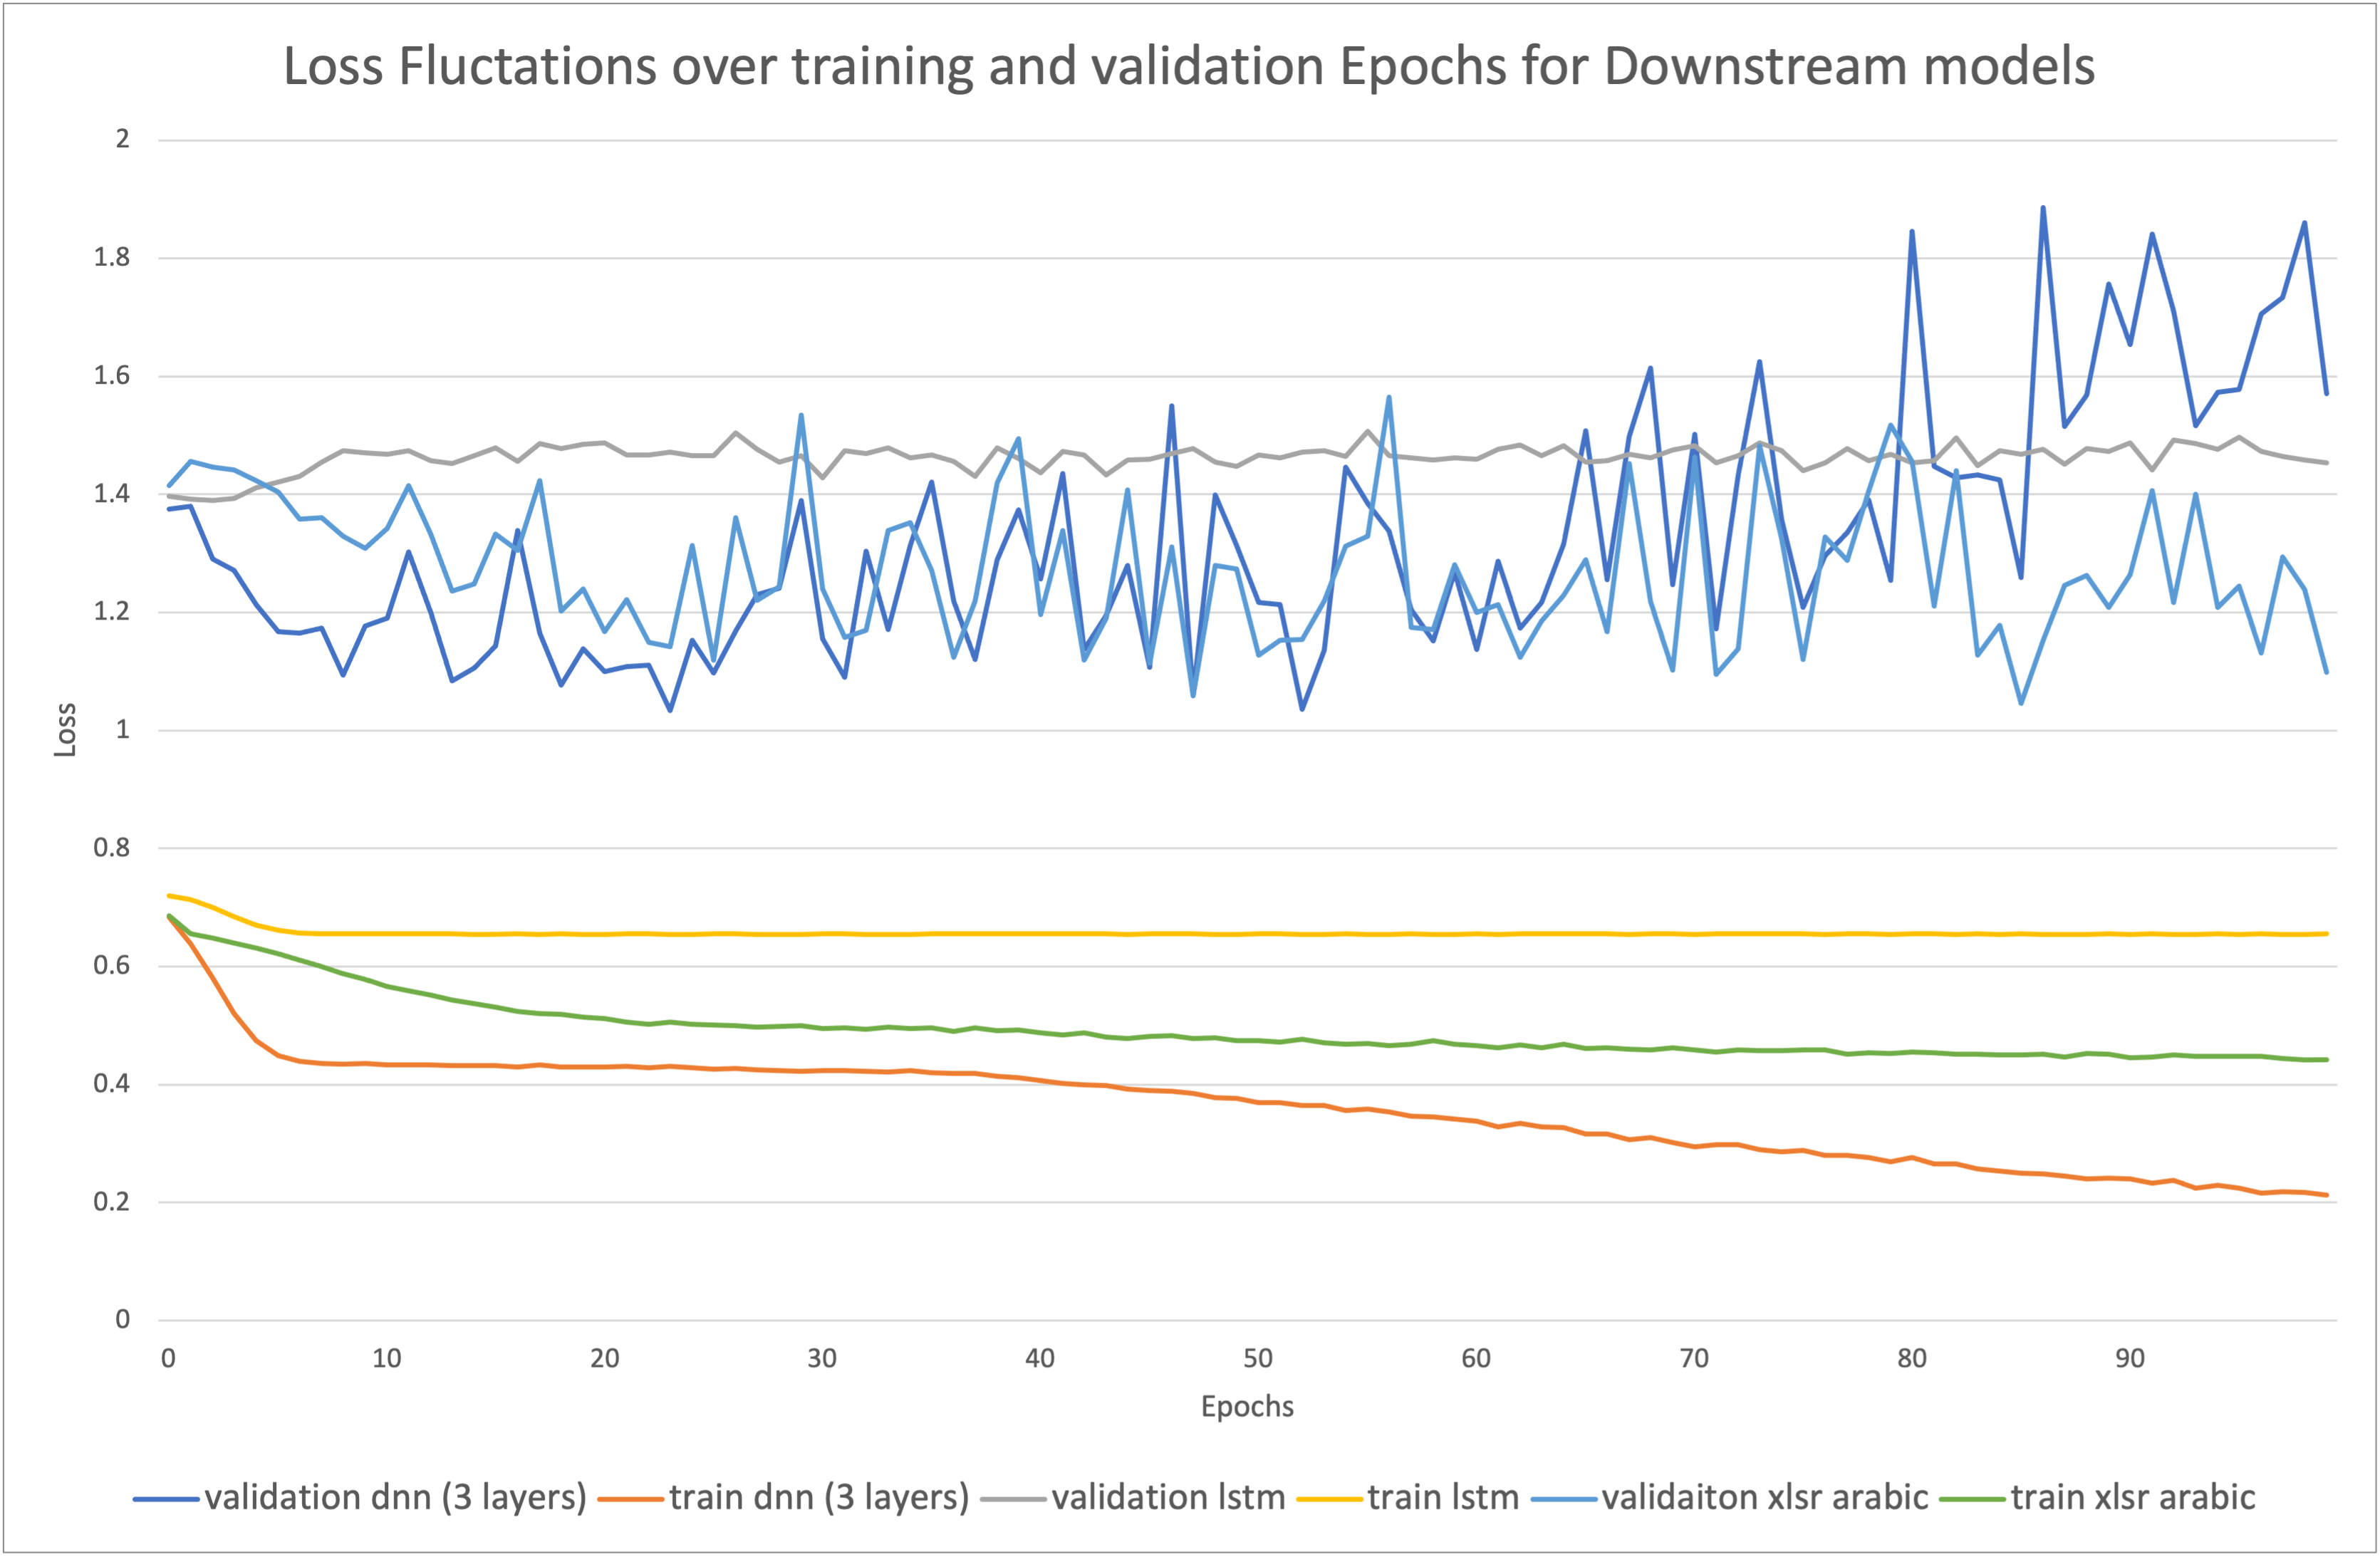
\includegraphics[width=\textwidth]{plots/downstreamLoss.png}
    \caption{Downstream model types change of loss.}
    \label{fig:downLoss}
\end{figure}

\subsection{Fine-tuning with Encoder layers}\label{sect:encoderExp}
A significant portion of the wav2vec pretrained model structure its encoder layers. 
Wav2vec and thereby XLSR Arabic has 12 encoder layers, in previous experimentation these layers were frozen. This portion of experimentation  
explores unfreezing those layers gradually while the model is fine-tuning.The training used the XSLR Arabic pretrained model with 3 GPUs, 24 CPUs, 138GB of memory 
and 700 files allocated per dialect. The step at which the layers are unfrozen is varied 
in testing and the results are shown in the Figure \ref{fig:unfreezeplot}. Analysing these results it was found that increases the 
step also increased the F1-Score until step 50 in which the F1-Score began to plateau and decrease. 
The highest F1-Scores overall was when the unfreezing step was set to 50 with a weighted average F1-Score of 76\%, it performed well on most dialects 
with the highest being North African (NOR) at 85\% and struggling with Egyptian with an F1-Score of 63\%. This model was the most effective umbrella DID developed out of 
all the experiments, it's final classification report is shown in Table \ref{tab:F1Score50freeze} and confusion matrix colour map in Figure \ref{fig:colour50UmbDID}. 

\begin{figure}[h!]
    \centering
    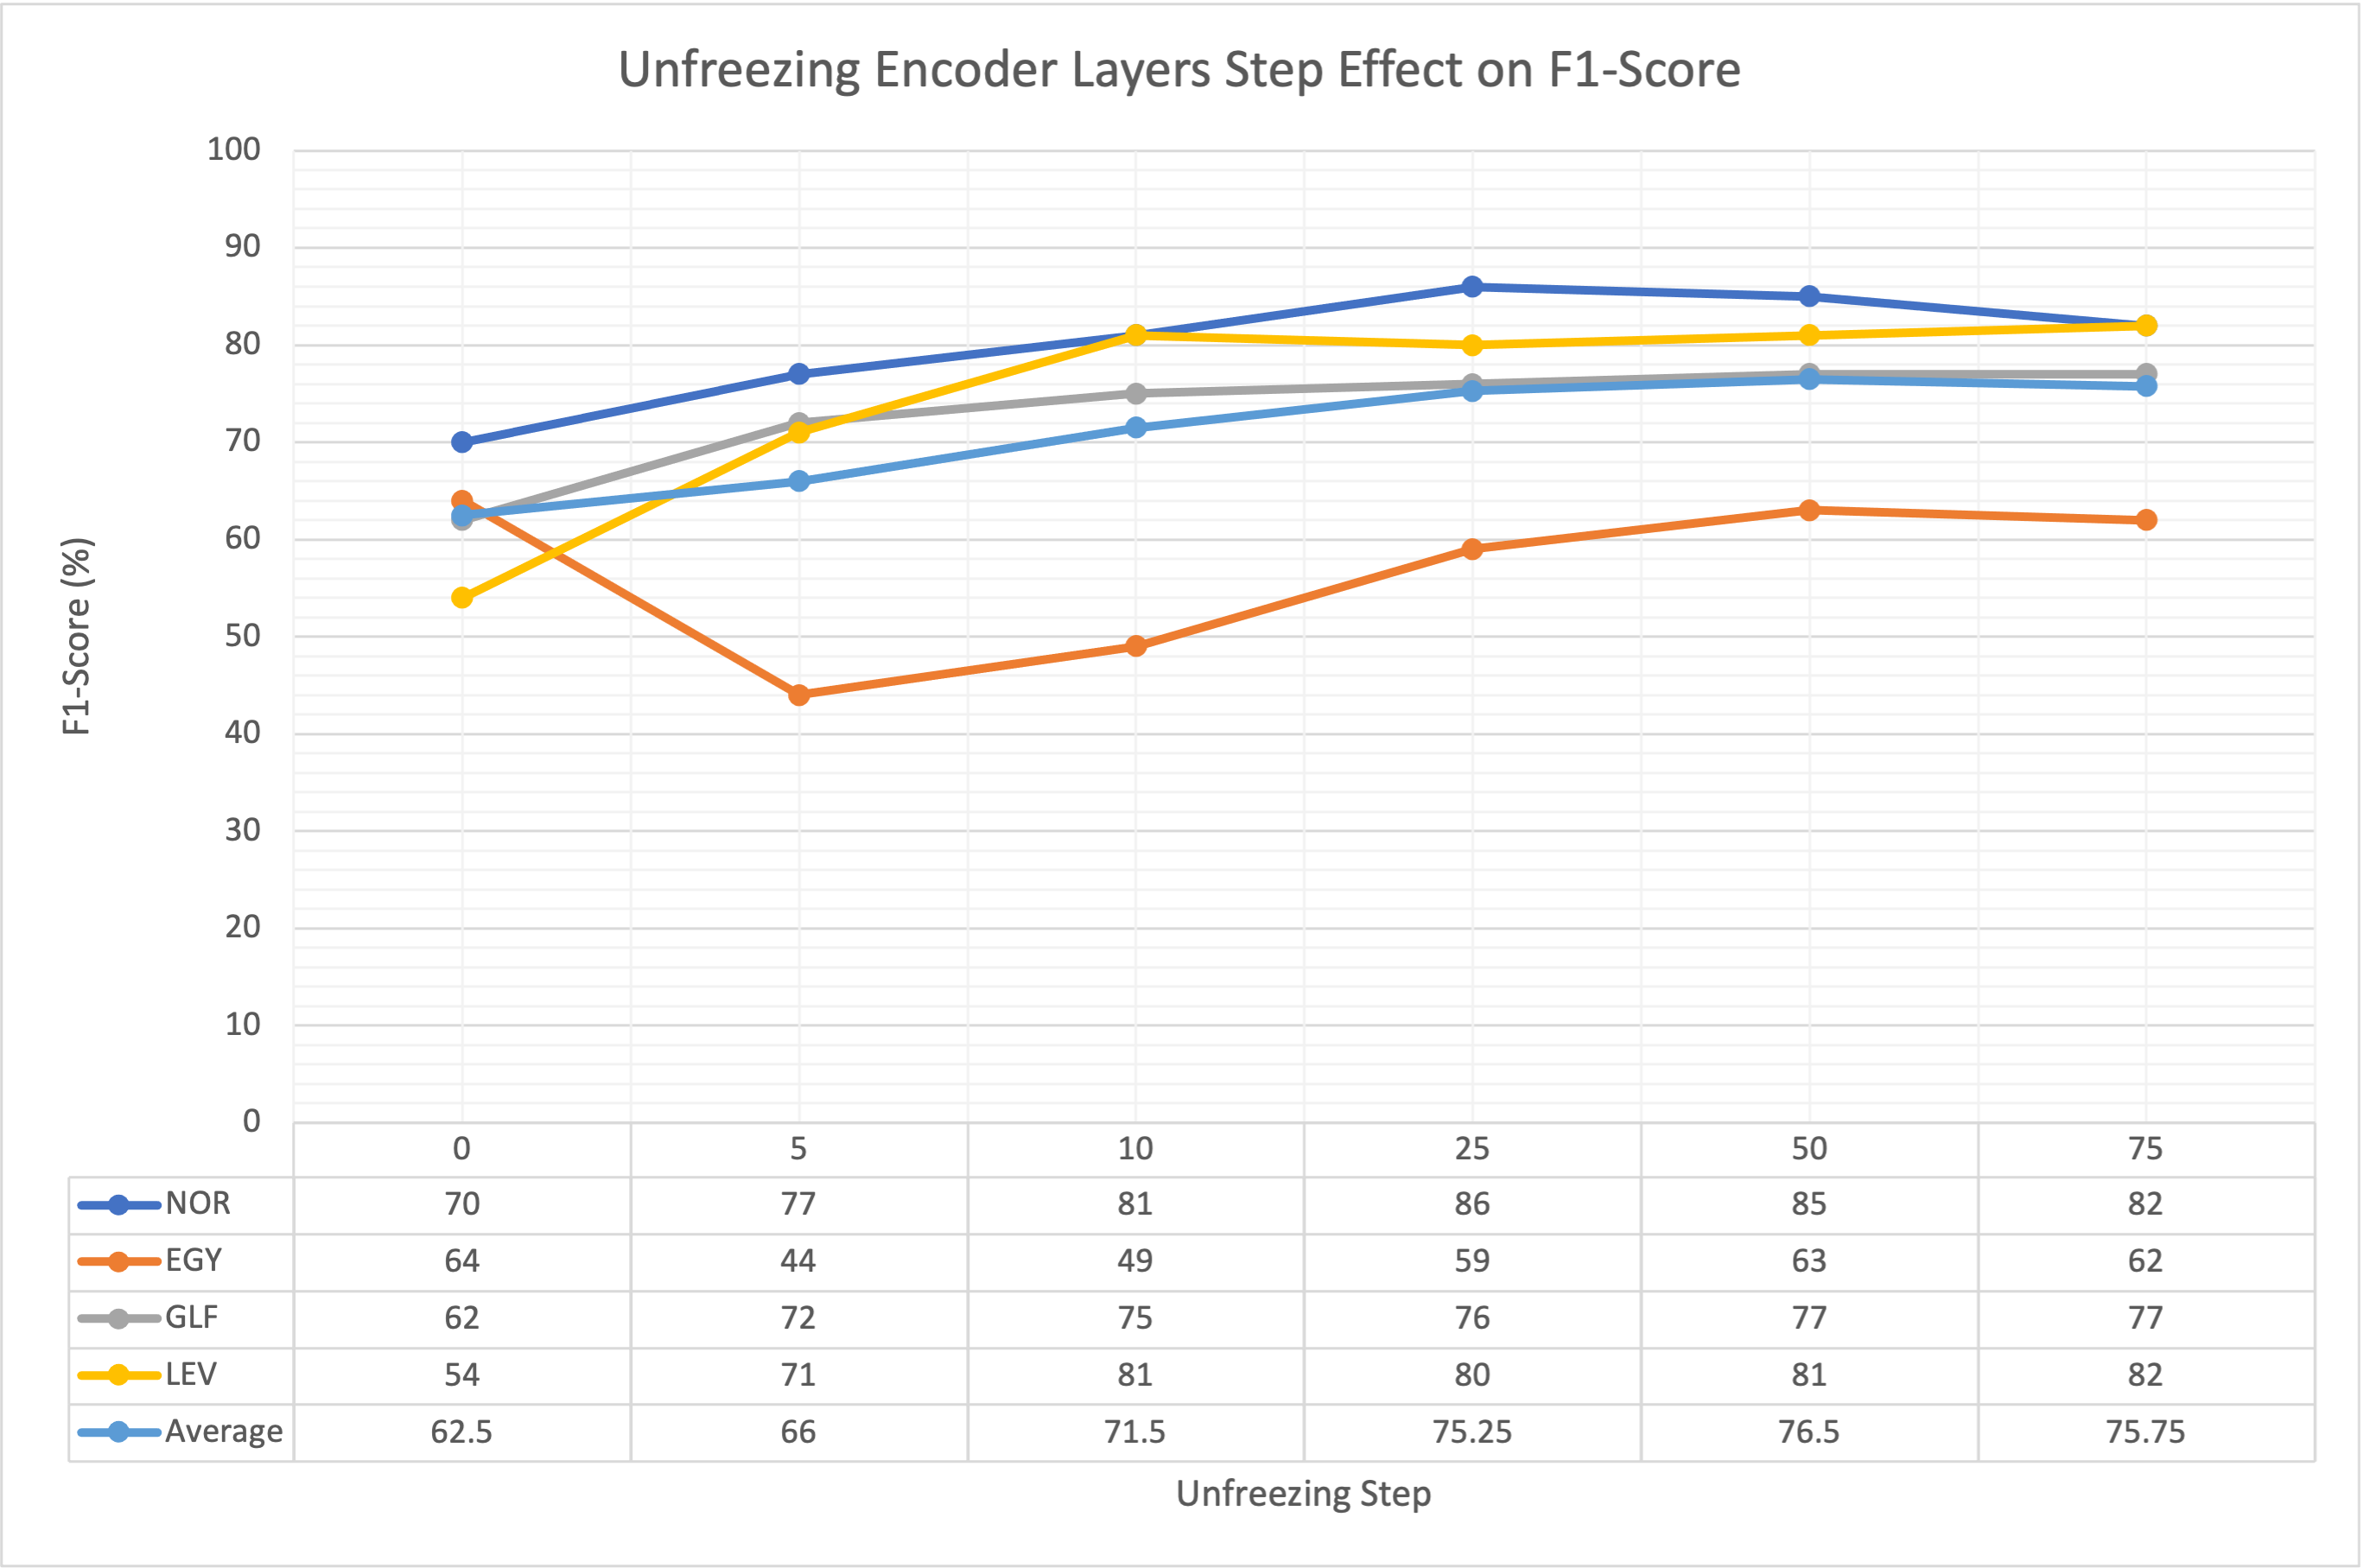
\includegraphics[width=\textwidth]{plots/unfreezegraph.png}
    \caption{Plot showing unfreeze encoder layer step effect on F1-Score. }
    \label{fig:unfreezeplot}
\end{figure}

\begin{table}[h!]
    \centering
    \label{tab:F1Score50freeze}
    \begin{tabular}{|l|l|l|l|l|} 
    \hline
                              & \textbf{Precision (\%)} & \textbf{Recall (\%)} & \textbf{F1-Score (\%)} & \textbf{Support}  \\ 
    \hline
    NOR                       & 86                      & 84                   & 85                     & 100               \\ 
    \hline
    EGY                       & 79                      & 52                   & 63                     & 100               \\ 
    \hline
    GLF                       & 69                      & 86                   & 77                     & 100               \\ 
    \hline
    LEV                       & 76                      & 86                   & 81                     & 100               \\ 
    \hline
    \textbf{Accuracy}         &                         &                      & 77                     & 400               \\ 
    \hline
    \textbf{Macro Average}    & 78                      & 77                   & 76                     & 400               \\ 
    \hline
    \textbf{Weighted Average} & 78                      & 77                   & 76                     & 400               \\
    \hline
\end{tabular}
\end{table}

\begin{figure}[h!]
    \centering
    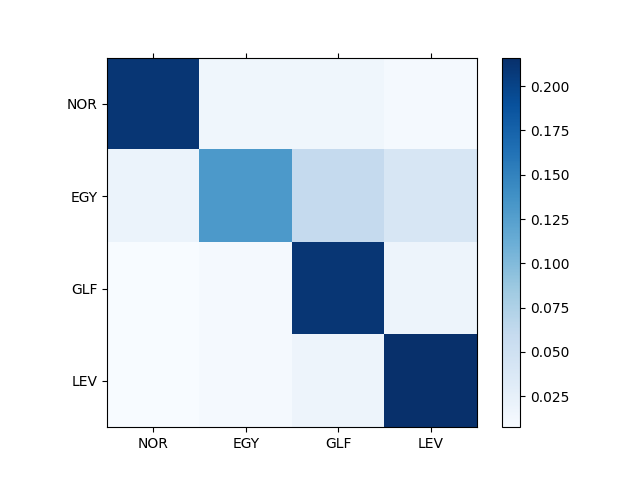
\includegraphics[height=10cm]{plots/ADI17-xlsr-araic-unfreeze-step50-norm.png}
    \caption{Step 50 Umbrella DID Normalised Confusion Matrix Colour Map.}
    \label{fig:colour50UmbDID}
\end{figure}

\section{Counteracting Data Bias}\label{sect:dataBias}
Two tests were conducted to observe the significance of biases from the pretrained model on the final model's performance. 
As well as testing to see if these biases could be counteracted by providing a disproportionate amount of data per dialect in 
the fine-tuning files. The training used the XSLR Arabic pretrained model with 3 GPUs, 24 CPUs, 138GB of memory 
and 700 files allocated for each of the unmodified dialects. 

\subsubsection{Fine-tuning without Levantine Arabic}
Inherited from the XLSR Arabic's pretraining is a data bias towards Levantine Arabic. 
To test the effects of this bias on the performance of the umbrella DID all training, validation and test files from the 
Levantine dialect were withheld from the pipeline. The hypothesis was that if the F1-Scores significantly improved, 
the bias inherited from the pretrained model may have limited the performance of the DID. Looking at the normalised 
colour map \ref{fig:NoLEV} and the results in the Table \ref{tab:f1bias} it can be seen that removing Levantine did not improve the F1-Score. 
Removing Levantine decreased the F1-Score of North African (NOR) identification by 17\%, misidentifying the audio clips as Egyptian (EGY) 22.8\% and Gulf (GLF) 38.9\% of the time. 
Whilst the weighted average F1-Score without Levantine was 71\%, 5\% less than the standard set of data with an average of 76\%. 
Hence, it was found that the bias from the pretrained model was not significant in determining the final performance of the Umbrella DID. 

\subsubsection{Fine-tuning with double the amount of Egyptian Arabic}
It was observed in Figure \ref{fig:colour50UmbDID} that the umbrella DID was challenged the most with identifying the Egyptian (EGY) dialect 
from the other umbrella dialects. It was proposed that doubling the training data given to the system to fine-tune the model could 
improve its performance. The training data provided for Egyptian was increased from 700 files to 1400. Although, observing the results in the Table 
\ref{tab:f1bias} and the Figure \ref{fig:x2EGY}, it can be seen that this doesn't improve the performance model. Increasing the Egyptian (EGY) data increases 
the F1-Score of Egyptian from 63\% to 78\% but the F1-Scores for all the other dialects decrease. The greatest drop in F1-Score can be seen in North African (NOR) going from 
85\% to 69\%. So, increasing the data for a particular class does not improve the system's ability to identify that class. 

\begin{table}
    \centering
    \label{tab:f1bias}
    \caption{Exploring Counteracting Data Biases }
    \begin{tabular}{|l|l|l|l|} 
    \hline
    \multicolumn{4}{|c|}{\textbf{ F-1 Score (\%)}}                    \\ 
    \hline
                              & No Adjustments & No LEV & Double EGY  \\ 
    \hline
    NOR                       & 85             & 68     & 69          \\ 
    \hline
    EGY                       & 63             & 68     & 78          \\ 
    \hline
    GLF                       & 77             & 73     & 61          \\ 
    \hline
    LEV                       & 81             & 72     & 66          \\ 
    \hline
    \textbf{Weighted Average} & 76             & 71     & 70          \\
    \hline
    \end{tabular}
    \end{table}

\begin{figure}[h!]
    \CommonHeightRow{
        \begin{floatrow}[2]
            \ffigbox[\FBwidth]
            {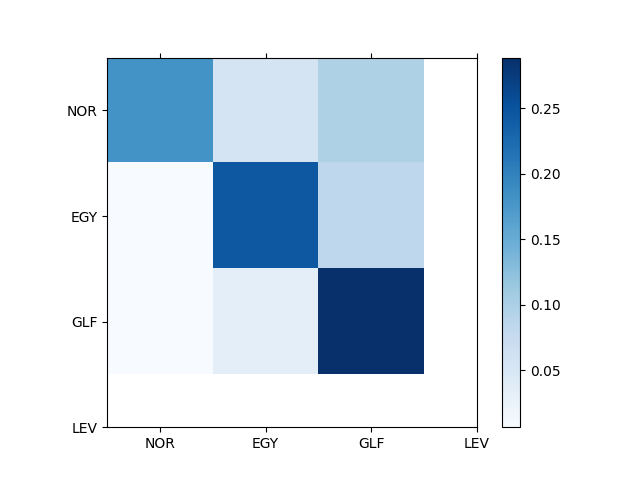
\includegraphics[height=6cm]{plots/ADI17-xlsr-araic-unfreeze-nolev-norm.png}}
            {\caption{No Levantine Normalised\newline Confusion Matrix Colour Map.}}\label{fig:NoLEV}
            \ffigbox[\FBwidth]
            {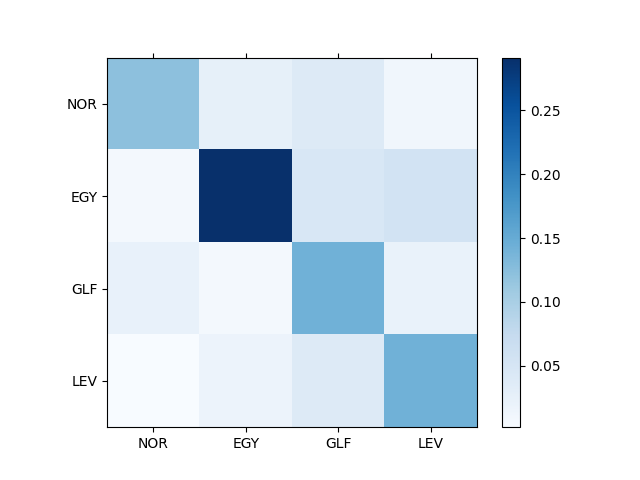
\includegraphics[height=6cm]{plots/ADI17-xlsr-araic-unfreeze-x2EGY-norm.png}}
            {\caption{Doubled Egyptian Training\newline Data Normalised Confusion Matrix Colour Map.}}\label{fig:x2EGY}
        \end{floatrow}}
\end{figure}

\pagebreak
\section{Assessing Robustness}
Through the process of developing the highest performance Umbrella DID design was the XLSR Arabic model with the encoder layers fined tuned at step 50. 
Taking this model its robustness is then tested by observing the minimum amount of training files needed to fine tune the model. As well as assessing how 
well the model performs when the trained model is then further fine-tuned for the downstream task of a regional dialect identifier. 
\subsection{Amount of Training Data}\label{sect:MinTrainingData}
Using 3 GPUs, 24 CPUs, 138GB of memory, the umbrella DID was fine-tuned with file amounts ranging from 25 to 1000. In the Figure 
\ref{fig:numFilesF1Score} it can be seen that the F1-Score doubles between 25 and 50 training files per dialect, going from a weighted average F1-Score 
of 26\% to 42\%. The F1-Score plateaus slightly and increases slowly between 200 and 400 files. Then significantly increasing at 600 to a weighted average F1-Score of 
66\% before plateauing again. From this it can be attained that it is sufficient to provide around 600 files per class without the model's performance fluctuating significantly. 
\begin{figure}[h!]
    \centering
    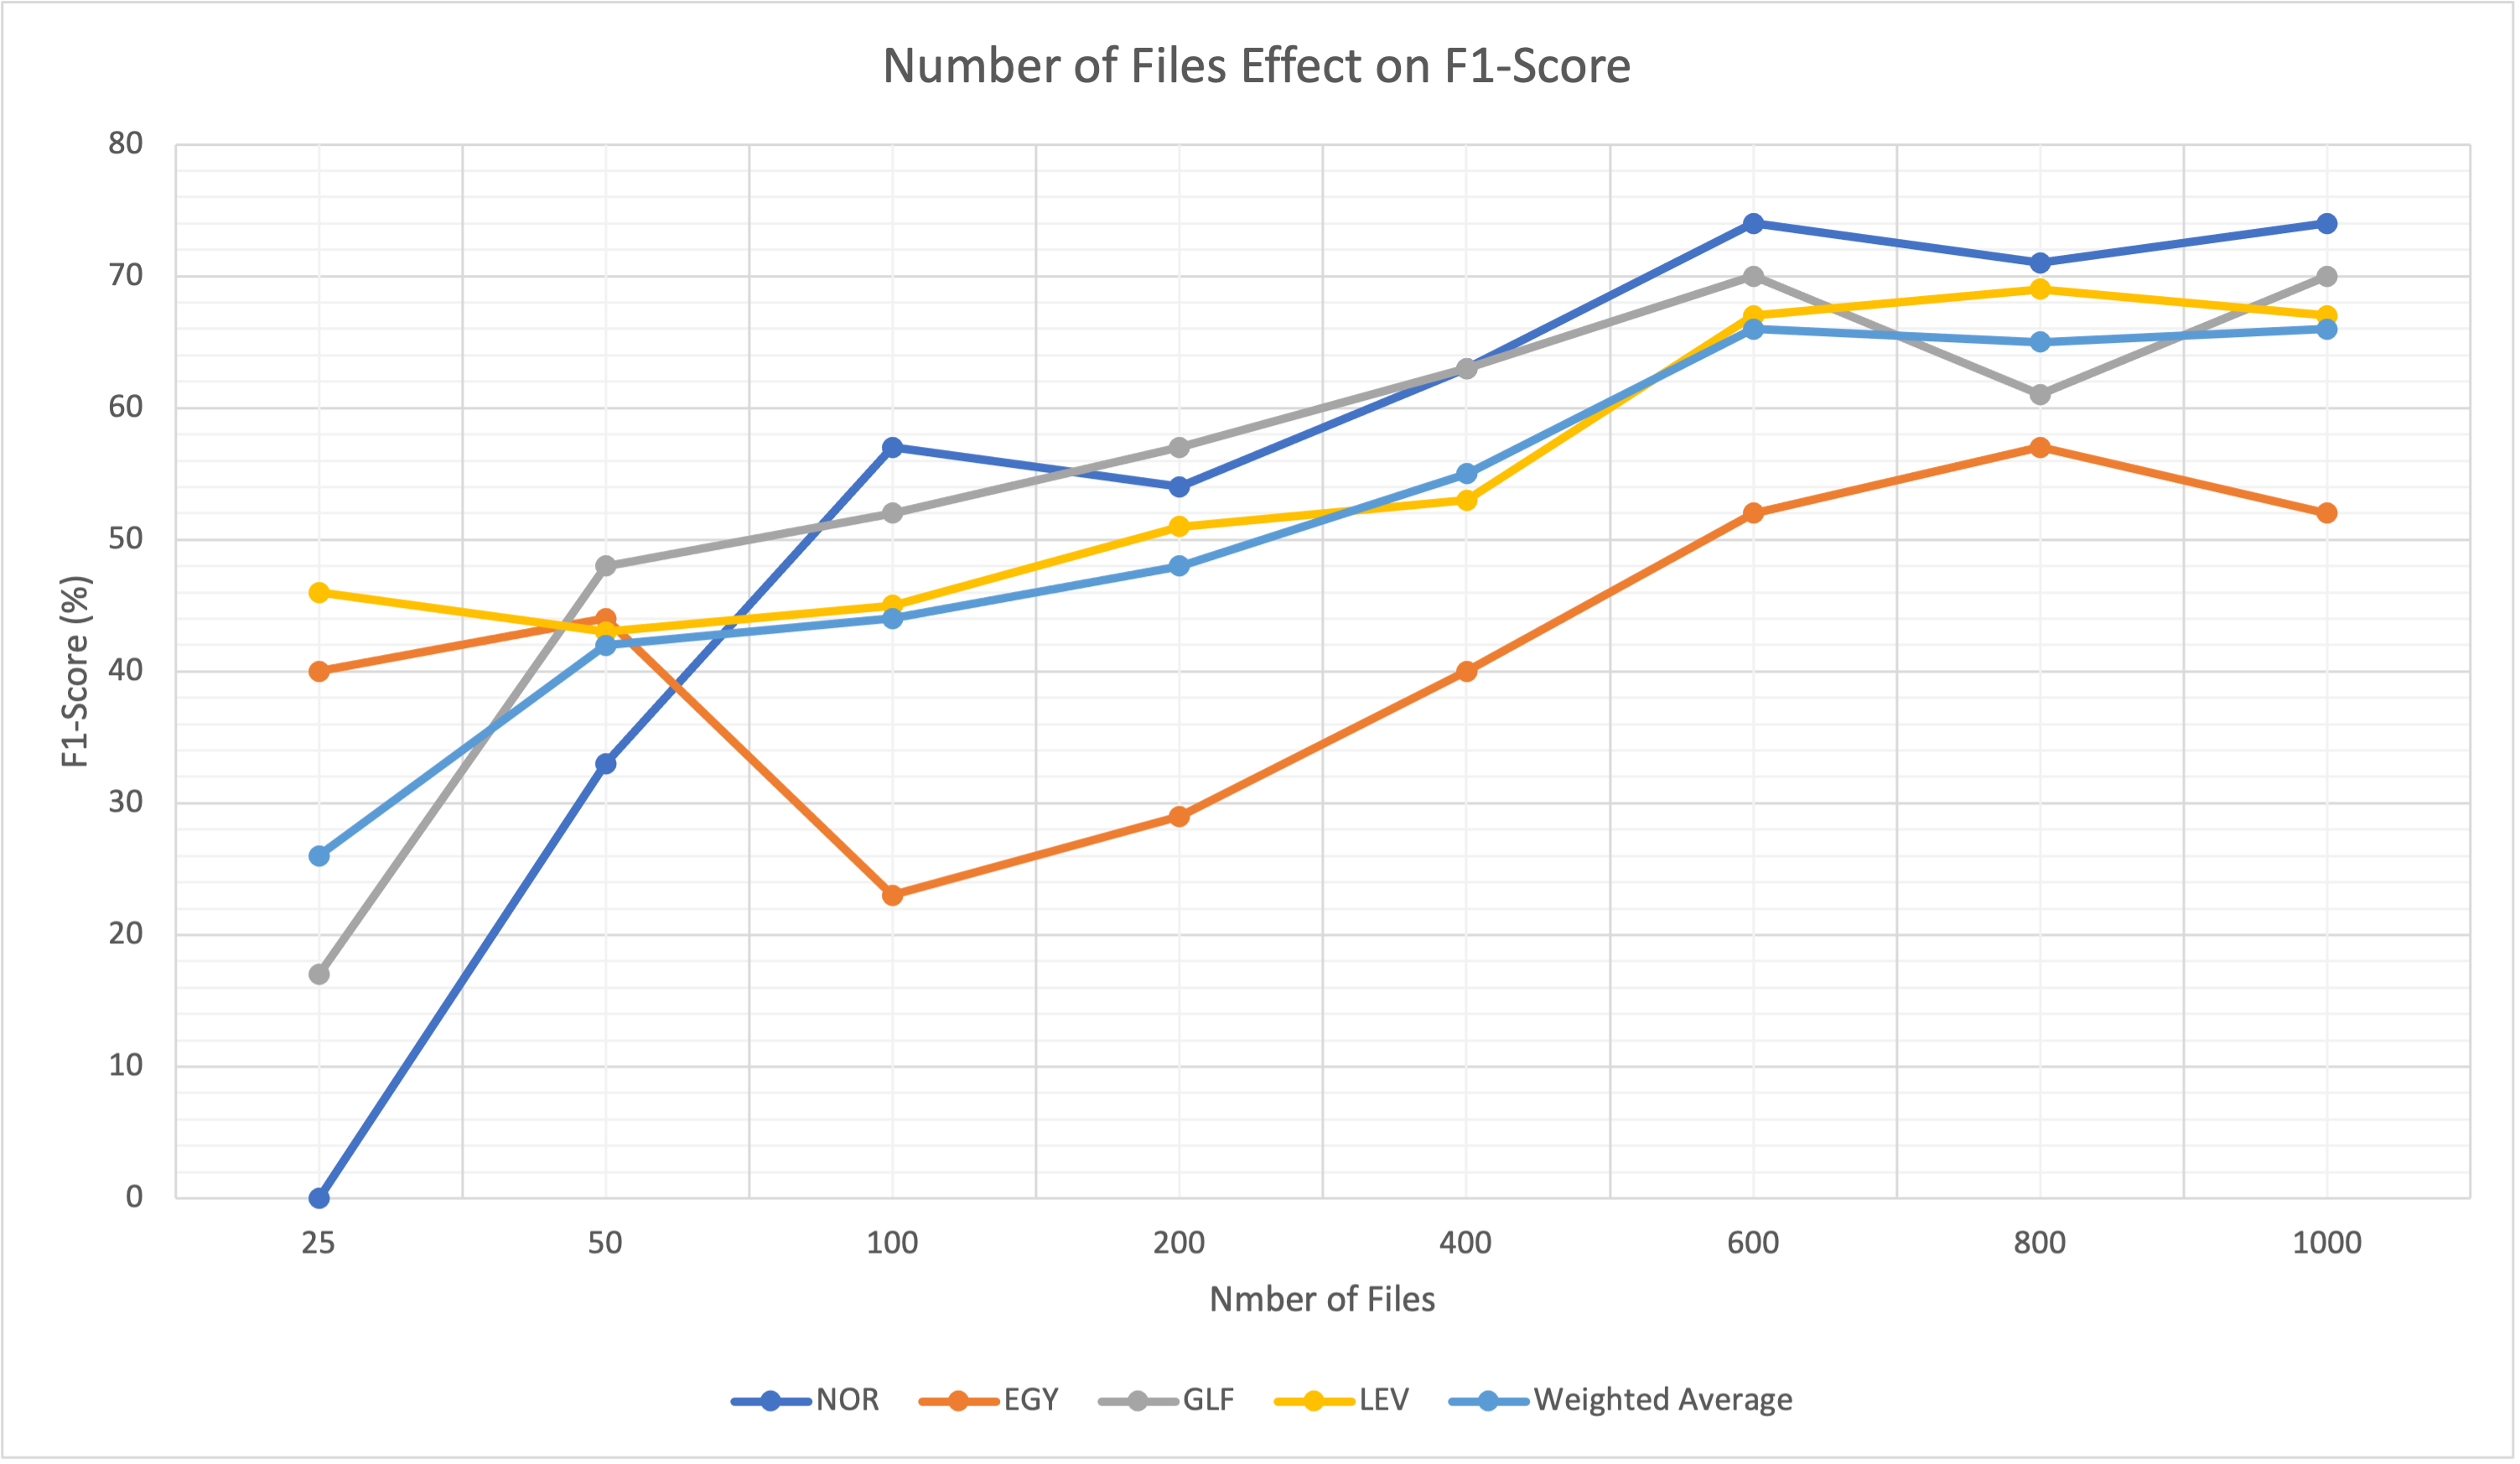
\includegraphics[height=10cm]{plots/numFilesF1Score.png}
    \caption{Number of Training Files Effect on F1-Score.}
    \label{fig:numFilesF1Score}
\end{figure}

\begin{table}[h!]
    \label{tab:f1numfiles}
    \centering
    \caption{F1-Scores of Varying Amounts of Training Files}
    \begin{tabular}{|l|l|l|l|l|l|l|l|l|} 
    \hline
                              & \multicolumn{8}{c|}{\textbf{F-1 Score (\%)~}}                                                                         \\ 
    \hline
    \textbf{Number of Files}  & \textbf{25} & \textbf{50} & \textbf{100} & \textbf{200} & \textbf{400} & \textbf{600} & \textbf{800} & \textbf{1000}  \\ 
    \hline
    NOR                       & 0           & 33          & 57           & 54           & 63           & 74           & 71           & 74             \\ 
    \hline
    EGY                       & 40          & 44          & 23           & 29           & 40           & 52           & 57           & 52             \\ 
    \hline
    GLF                       & 17          & 48          & 52           & 57           & 63           & 70           & 61           & 70             \\ 
    \hline
    LEV                       & 46          & 43          & 45           & 51           & 53           & 67           & 69           & 67             \\ 
    \hline
    \textbf{Weighted Average} & 26          & 42          & 44           & 48           & 55           & 66           & 65           & 66             \\
    \hline
    \end{tabular}
    \end{table}

\subsection{Adaptability to Regional DID}\label{sect:regDID}
The final test conducted was testing the DID's adaptability to being used in a finer grain dialect identifying task. The number of classes 
on the output layer were increased from 4 to 17. The model was then trained on 3 GPUs, 24 CPUs, 138GB of memory with 700 files per dialect making the total number of training files 11900. 
As seen in the classification report in Table \ref{tab:regDIDclassifaction}, the final weighted average F1-Score of the regional DID was 58\% with the model performing better on some 
dialects more than others. The Regional Arabic DID excelled at identifying Iraqi (IRQ) Arabic with an F1-Score of 96\% while struggling the most with Egyptian (EGY), Sudan (SDN), Saudi (SAU) and Algerian (DZA).
Inspecting the miss identifications \ref{fig:colourRegDID}, Saudi (SAU) was most likely to misidentified as KWT, ARE, QAT OMN and YEM, all of which are in the Gulf region. This misidenfication from a dialect regionally 
close is also seen with Algerian (DZA) which is most likely to be misidentified as Moroccan (MAR). From this it can be inferred that the regional DID while working well for more distinct dialects finds it 
challenging to differentiate linguistically similar regional dialects.  


\begin{figure}[h!]
    \centering
    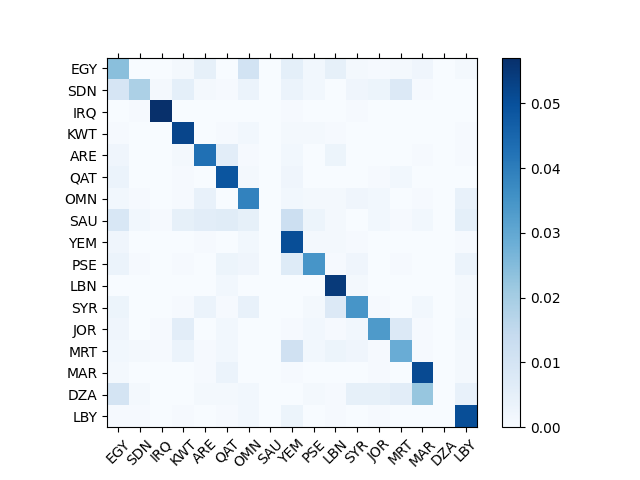
\includegraphics[height=10cm]{plots/ADI17-xlsr-regional-unfreeze-norm.png}
    \caption{Regional DID Normalised Confusion Matrix Colour Map.}
    \label{fig:colourRegDID}
\end{figure}

\begin{table}[h!]
    \centering
    \label{tab:regDIDclassifaction}
    \caption{Regional DID Classification Report}
    \begin{tabular}{|l|l|l|l|l|} 
    \hline
    \multicolumn{5}{|l|}{\textbf{CLASSIFICATION REPORT }}                \\ 
    \hline
                              & Precision & Recall & F1-Score & Support  \\ 
    \hline
    EGY                       & 32\%      & 41\%   & 36\%     & 100      \\ 
    \hline
    SDN                       & 74\%      & 32\%   & 45\%     & 100      \\ 
    \hline
    IRQ                       & 95\%      & 97\%   & 96\%     & 100      \\ 
    \hline
    KWT                       & 68\%      & 89\%   & 77\%     & 100      \\ 
    \hline
    ARE                       & 66\%      & 73\%   & 69\%     & 100      \\ 
    \hline
    QAT                       & 64\%      & 83\%   & 72\%     & 100      \\ 
    \hline
    OMN                       & 53\%      & 66\%   & 59\%     & 100      \\ 
    \hline
    SAU                       & 0\%       & 0\%    & 0\%      & 100      \\ 
    \hline
    YEM                       & 50\%      & 86\%   & 63\%     & 100      \\ 
    \hline
    PSE                       & 69\%      & 59\%   & 63\%     & 100      \\ 
    \hline
    LBN                       & 69\%      & 93\%   & 79\%     & 100      \\ 
    \hline
    SYR                       & 64\%      & 59\%   & 61\%     & 100      \\ 
    \hline
    JOR                       & 70\%      & 57\%   & 63\%     & 100      \\ 
    \hline
    MRT                       & 53\%      & 49\%   & 51\%     & 100      \\ 
    \hline
    MAR                       & 62\%      & 87\%   & 72\%     & 100      \\ 
    \hline
    DZA                       & 0\%       & 0\%    & 0\%      & 100      \\ 
    \hline
    LBY                       & 66\%      & 86\%   & 74\%     & 100      \\ 
    \hline
    \textbf{Accuracy}         &           &        & 62\%     & 1700     \\ 
    \hline
    \textbf{Macro Average}    & 56\%      & 62\%   & 58\%     & 1700     \\ 
    \hline
    \textbf{Weighted Average} & 56\%      & 62\%   & 58\%     & 1700     \\
    \hline
    \end{tabular}
    \end{table}

\pagebreak 
\section{Summary of Results}\label{sect:sumResults}
Comparing the performance of the umbrella and regional DID construct in this thesis to traditional methods. 
It was found that a pretrained model and a transfer learning approach to designing a regional DID under performed with an accuracy of 62\% compared to the paper  \cite{lin_transformer-based_2020} in where they were able to achieve an accuracy of 85.1\% . 
Although, in comparison to a phonetic approach discussed in the paper \cite{biadsy_spoken_2009}, the transfer learning approach was able to achieve higher F1-Scores with 10s utterances. As shown in Table \ref{tab:comparision} the transfer learning DID 
design in this thesis had a higher F1-Score for Levantine (LEV) by 3\%, Gulf (GLF) by 21\% and Iraqi (IRQ) by 40\%. With only Egyptian (EGY) being better represented through the phonetic approach with it's F1-Score of 84\% compared to the 
transfer learning's 63\%. 

\begin{table}[h!]
    \centering
    \label{tab:comparision}
    \caption{Regional DID Classification Report}
    \begin{tabular}{|l|l|l|} 
    \hline
    \multicolumn{3}{|c|}{F1-Score (\%)}                 \\ 
    \hline
        & Transfer Learning DID~ & Phonematic Model \cite{biadsy_spoken_2009} \\ 
    \hline
    LEV & 81                     & 78                   \\ 
    \hline
    GLF & 77                     & 56                   \\ 
    \hline
    EGY & 63                     & 84                   \\ 
    \hline
    IRQ & 96                     & 56                   \\
    \hline
    \end{tabular}
    \end{table}

Finally, to summarise the findings of the experimentation conducted during this thesis and presented in this chapter: 
\begin{enumerate}
\item It was found that a pretrained model that was pretrained with data similar to the downstream task 
was effective approach to transfer learning, although adapting pretrained models fine-tuned on similar downstream tasks also showed promise. 
In the case explored in this thesis in designing an Arabic DID, XLSR Arabic, a pretrained model that was pretrained on 53 languages and Levantine Arabic produced the most successful DID model. (Section \ref{sect:pretrainExp})
\item Removing noise from input files did not improve the performance of pipelines due to the distortions it caused to the audio. (Section \ref{sect:noiseExp})
\item Longer utterance lengths were more accurate but using files longer than 10s was unsustainable with the resources available as longer audio clips were not able to be processed in a timely manner. (Section \ref{sect:uttExp})
\item Unfreezing and fine-tuning encoder layers for the last 50 epochs improved the system significantly. (Section \ref{sect:encoderExp})
\item Including a downstream model showed promise, but the added complexity to the system created diminishing returns in improvement. (Section \ref{sect:downExp})
\item Inherited biases from the pretrained don't have a significant effect on the final performance of the Arabic DID systems and training with unbalanced amount of data 
was not effective at correcting performance differences between the dialect classes. (Section \ref{sect:dataBias})
\item The minimum amount of training data needed to effectively train an Arabic DID is around 500 files although significant improvements to the transfer learning DID's performance for this result to be conclusive (Section \label{sect:MinTrainingData})
\end{enumerate}